\documentclass[12pt,a4paper,oneside]{book}

\usepackage{a4wide}                     % Iets meer tekst op een bladzijde
\usepackage[dutch,english]{babel}       % Voor nederlandstalige hyphenatie (woordsplitsing)
\usepackage{amsmath}                    % Uitgebreide wiskundige mogelijkheden
\usepackage{amssymb}                    % Voor speciale symbolen zoals de verzameling Z, R...
\usepackage{url}                        % Om url's te verwerken
\usepackage{graphicx}                  % Om figuren te kunnen verwerken
\usepackage[small,bf]{caption}    % Om de captions wat te verbeteren
\usepackage{xspace}                     % Magische spaties na een commando
\usepackage[utf8]{inputenc}           	% Om niet ascii karakters rechtstreeks te kunnen typen
\usepackage{float}                      % Om nieuwe float environments aan te maken. Ook optie H!
\usepackage{flafter}                    % Opdat floats niet zouden voorsteken
\usepackage{listings}                   % Voor het weergeven van letterlijke text en codelistings
\usepackage{marvosym}                   % Om het euro symbool te krijgen
\usepackage{textcomp}                   % Voor onder andere graden celsius
\newcommand{\textapprox}{\raisebox{0.5ex}{\texttildelow}}
\usepackage{fancyhdr}                   % Voor fancy headers en footers.
\usepackage{graphics}					% Om figuren te verwerken.
\usepackage[nottoc]{tocbibind} 			% Bibliografie in ToC; zie tocbibind.dvi
%\usepackage{pstricks}
\usepackage{longtable}
\usepackage{pdfpages}  					% pdf pagina's importeren
\usepackage[numbers]{natbib}			% Extra citeer mogelijkheden
\usepackage{parskip}					% Geen indentatie bij begin paragraaf
\usepackage[hang,flushmargin,bottom]{footmisc} % Voetnoten beter weergeven (niet laten splitsen)
\usepackage{enumitem} 					%Betere opsommingen
\usepackage{sidecap}  					%Caption lang
\usepackage[toc,page]{appendix} 		%Appendices toevoegen
\usepackage{tikz}						%Toevoegen van tikz figuren
\usepackage{pgfplots}					%Grafieken plotten in tikz figuren
\usepackage{amsmath}
\usepackage{tikzscale}
\usepackage{environ}
\usepackage{authblk} 
\usetikzlibrary{arrows}
\usepackage{wrapfig}					%Figuren wrappen
\usepackage{subfig}                     %Figuren naast elkaar floaten
\usepackage[simplified]{pgf-umlcd}					%Uml diagrammen maken
%Uml border color
\renewcommand{\umldrawcolor}{black}		

%Allow a different display name for packages, so it's possible to use dots.
\renewenvironment{package}[2][\umlcdPackageTitle]{
	\edef\umlcdPackageTitle{#2}
	\def\umlcdPackageFit{}
	\def\umlcdPackageName{#1}
}{
\begin{pgfonlayer}{background}
	\node[umlcd style, draw, inner sep=0.5cm, fit = \umlcdPackageFit] (\umlcdPackageName) {};
	\node[umlcd style, draw, outer ysep=-0.5, anchor=south west] (\umlcdPackageName caption) at
	(\umlcdPackageName.north west) {\umlcdPackageTitle};
\end{pgfonlayer}
}

\tikzset{
	template parameter/.style={
		append after command={
			node [draw, densely dashed, umlcolor, font=\ttfamily]
			at (\tikzlastnode.north east)
			{#1}
		}
	}
}

%Better underlining
\usepackage{soul}
%pseudocode tonen
\usepackage{algorithm,algpseudocode}
\usepackage{setspace}

%Marge onderaan wat vergroten
\setlength{\textheight}{660pt}

%Package om geometrie overzicht van document te tonen.
%\usepackage{layout}

\interfootnotelinepenalty=10000

\newcommand{\npar}{\par \vspace{2.3ex plus 0.3ex minus 0.3ex} \noindent}	% Om witruimte te krijgen tussen paragrafen
\graphicspath{{figuren/}}               % De plaats waar latex zijn figuren gaat halen.
%\usepackage[bf]{caption2}				% Mooiere captions
\usepackage[a4paper,plainpages=false]{hyperref}    % Om hyperlinks te hebben in het pdfdocument.

\newcommand{\command}[1]{\lstinline[basicstyle=\tt]{#1}\xspace} %Voor commando's
\hyphenation{tijd-as audio-stream} 							% Splitsing van woorden

\renewcommand{\chaptermark}[1]{\markright{\MakeUppercase{#1}}}
\renewcommand{\sectionmark}[1]{\markright{\thesection~#1}}

\newcommand{\headerfmt}[1]{\textsl{\textsf{#1}}}
\newcommand{\headerfmtpage}[1]{\textsf{#1}}

\fancyhf{}
\fancyhead[LE,RO]{\headerfmtpage{\thepage}}
\fancyhead[LO]{\headerfmt{\rightmark}}
\fancyhead[RE]{\headerfmt{\leftmark}}
\renewcommand{\headrulewidth}{0.5pt}
\renewcommand{\footrulewidth}{0pt}

\fancypagestyle{plain}{ % eerste bladzijde van een hoofdstuk
	\fancyhf{}
	\fancyhead[LE,RO]{\headerfmtpage{\thepage}}
	\fancyhead[LO]{\headerfmt{\rightmark}}
	\fancyhead[RE]{\headerfmt{\leftmark}}
	\renewcommand{\headrulewidth}{0.5pt}
	\renewcommand{\footrulewidth}{0pt}
}

\renewcommand{\lstlistoflistings}{\begingroup
	\tocfile{\lstlistlistingname}{lol}
	\endgroup}


% anderhalve interlinie (opm: titelblad gaat uit van 1.5)
\renewcommand{\baselinestretch}{1.5}


%Pdf instellen, links, meta info
\hypersetup {
	pdfauthor = {Ward Van Assche},
	pdftitle = {Realtime signaal synchronisatie	met accoustic fingerprinting},
	pdfsubject = {Masterproef ingediend tot het behalen van de academische graad van Master of Science in de industriële wetenschappen: informatica, juni 2016},
	colorlinks = False,
%	pdfborder = {0 0 0}
}

%Titels wijzigen in correcte Nederlandse term
\renewcommand\lstlistlistingname{Lijst van codefragmenten}
\renewcommand\lstlistingname{Codefragment}
\addto{\captionsdutch}{
	\renewcommand{\bibname}{Referentielijst}
	\renewcommand\appendixname{Bijlage}
	\renewcommand\appendixpagename{Bijlagen}
	\renewcommand\appendixtocname{Bijlagen}
}

\begin{document}
\selectlanguage{dutch}

%officieel Plato titelblad
\includepdf[pages=-]{./titelblad.pdf}

% titelblad (voor kaft)
%  Titelblad

% Opmerking: gaat uit van een \baselinestretch waarde van 1.5 (die moet
% ingesteld worden voor het begin van de document environment)

\begin{titlepage}

\setlength{\hoffset}{-1in}
\setlength{\voffset}{-1in}
\setlength{\topmargin}{1.5cm}
\setlength{\headheight}{0.5cm}
\setlength{\headsep}{1cm}
\setlength{\oddsidemargin}{3cm}
\setlength{\evensidemargin}{3cm}
\setlength{\footskip}{1.5cm}
\enlargethispage{1cm}
% \textwidth en \textheight hier aanpassen blijkt niet te werken

\fontsize{12pt}{14pt}
\selectfont

\begin{center}

\includegraphics[height=2cm]{ruglogo}

\vspace{0.5cm}

Faculteit Ingenieurswetenschappen en Architectuur\\
Vakgroep Informatietechnologie\\
Voorzitter: Prof.~Dr.~Ir.~Daniël De Zutter

\vspace{3cm}

\fontseries{bx}
\fontsize{17.28pt}{21pt}
\selectfont

Realtime signaal synchronisatie \\
met accoustic fingerprinting

\fontseries{m}
\fontsize{12pt}{14pt}
\selectfont

\vspace{.6cm}

door 

\vspace{.4cm}

Ward Van Assche

\vspace{2.5cm}

Promotoren: Dr.~Marleen Denert, Joren Six\\
Scriptiebegeleider: Prof.~Helga Naessens\\

\vspace{2cm}

Masterproef ingediend tot het behalen van de academische graad van\\
Master of Science in de industriële wetenschappen: informatica

\vspace{0.5cm}

Academiejaar 2015--2016

\end{center}
\end{titlepage}


% Invoegen van layout testpagina
% \layout

% lege pagina (!!)

% titelblad (!!)

% geen paginanummering tot we aan de inhoudsopgave komen
\pagestyle{empty}

% voorwoord met dankwoord en toelating tot bruikleen (ondertekend)
%  Voorwoord (dankwoord) en toelating tot bruikleen

\newpage

\noindent \textbf{\huge Voorwoord}

\vspace{1.5cm}

\noindent
Lorem ipsum dolor sit amet, consectetur adipiscing elit. Praesent ac tristique risus. Morbi sit amet porta ex. Vivamus at blandit mi, eget finibus nisi. Cum sociis natoque penatibus et magnis dis parturient montes, nascetur ridiculus mus. Nulla vehicula efficitur rutrum. Quisque ac condimentum ligula, at tempus leo. Sed quis felis erat. Proin volutpat et odio ac finibus. Cras eu ultrices augue. Aliquam finibus lacus ut erat placerat, non ullamcorper arcu porttitor. Phasellus nisi metus, porttitor pretium diam ac, euismod ultricies nunc. Proin auctor pulvinar tellus eu egestas. Fusce non nisl commodo, luctus diam a, interdum ex. Pellentesque quis enim sit amet felis suscipit suscipit sed ac nunc. Integer porta, ipsum non placerat tincidunt, est quam eleifend urna, sed aliquam libero felis ac odio.\\

Proin non maximus est. Nullam eu magna et mauris faucibus dictum. Vivamus vitae commodo enim, dignissim consequat magna. Vivamus et elementum velit. Suspendisse justo lacus, euismod in nibh nec, dictum eleifend libero. Vivamus dapibus dignissim nibh, eu luctus nunc. Vivamus hendrerit massa in velit cursus pharetra. Aliquam consectetur dapibus mi at semper. \\

Nam rhoncus lectus risus. Vivamus dolor justo, viverra nec libero eget, porttitor rhoncus sapien. Proin commodo erat leo, eget dignissim massa consequat non. Sed pharetra eget libero nec faucibus. \\

\addvspace{2.5cm}

\noindent Ward Van Assche, juni 2016\newpage

\noindent \textbf{\huge Toelating tot bruikleen}

\vspace{1.5cm}

\noindent
``De auteur geeft de toelating deze scriptie voor consultatie beschikbaar
te stellen en delen van de scriptie te kopi\"eren voor persoonlijk
gebruik.\\
Elk ander gebruik valt onder de beperkingen van het auteursrecht,
in het bijzonder met betrekking tot de verplichting de bron uitdrukkelijk
te vermelden bij het aanhalen van resultaten uit deze scriptie.''

\addvspace{4cm}

\noindent Ward Van Assche, juni 2016


% overzicht
%  Overzichtsbladzijde met samenvatting

\newpage

{
\setlength{\baselineskip}{14pt}
\setlength{\parindent}{0pt}
\setlength{\parskip}{8pt}

\begin{center}

\noindent \textbf{\huge
Realtime signaal synchronisatie\\[8pt]
met acoustic fingerprinting
}

door 

Ward Van Assche

Masterproef ingediend tot het behalen van de academische graad van\\
Master of Science in de industriële wetenschappen: informatica

Academiejaar 2015--2016

Promotoren: Dr.~Marleen Denert, Joren Six\\
Scriptiebegeleider: Prof.~Helga Naessens

Faculteit Ingenieurswetenschappen en Architectuur\\
Universiteit Gent

Vakgroep Informatietechnologie\\
Voorzitter: Prof.~Dr.~Ir.~Dani\"{e}l De Zutter


\end{center}

\section*{Samenvatting}

% TODO: samenvatting schrijven

De meeste experimenten die aan het IPEM worden uitgevoerd maken gebruik van verschillende soorten sensoren (accelerometers, druksensoren,...). Een veelvoorkomend probleem is de de synchronisatie van de data van elke sensor. Bij het huidige synchronisatiesysteem wordt elke sensor verbonden met een microfoon die het omgevingsgeluid opneemt. Met technieken zoals acoustic fingerprinting en het berekenen van de kruiscovariantie kan de latency tussen de audiosignalen zeer nauwkeurig bepaald worden. Met deze latency kan vervolgens de sensordata gesynchroniseerd worden. Het huidige systeem kan enkel als naverwerking uitgevoerd worden. Een realtime en meer gebruiksvriendelijk systeem is erg gewenst. In dit onderzoek is er nagegaan of dit mogelijk is. Om de huidige synchronisatiealgoritmen in realtime bruikbaar te maken waren aanpassingen en optimalisaties nodig. Dit onderzoek heeft ook geleid tot enkele Max/MSP modules. Met behulp van deze modules is het mogelijk om het volledige synchronisatieproces in realtime uit te voeren in zonder het schrijven van één lijn code.


\section*{Trefwoorden}

% TODO: trefwoorden

synchronisatie, sensoren, audio, geluid, realtime, signalen, streams, acoustic fingerprinting, kruiscovariantie, digitale signaalverwerking

}
\newpage % strikt noodzakelijk om een header op deze blz. te vermijden


% abstract pdf toevoegen
\addcontentsline{toc}{chapter}{Extended abstract}
\includepdf[pages=-]{../abstract/abstract.pdf}
\pagestyle{fancy}

\frontmatter

% inhoudstafel
\tableofcontents

% afkortingen
\chapter{Gebruikte afkortingen}
\begin{flushleft}
	\renewcommand{\baselinestretch}{1.5}
	\small\normalsize
	\begin{longtable}{ll}
		IPEM				&  Instituut voor Psychoakoestiek en Elektronische Muziek \\
		DSP					&  Digital Signal Processing \\
		FFT					&  Fast Fourier Transform \\
		SFT					&  Short Time Fourier Transform \\
		ECG					&  Elektrocardiogram \\
		DTW					&  Dynamic timewarping \\
		USB					&  Universal Serial Bus \\
		ADC					&  Analog-to-digital converter \\
		PCM					&  Pulse-code modulation
		
	\end{longtable}
\end{flushleft}

% hoofdstukken
\mainmatter


% hier worden de hoofdstukken ingevoegd (\includes)
\chapter{Inleiding}

\section{Probleemschets}

Het probleem dat in deze masterproef zal worden onderzocht doet zich heel specifiek voor bij verschillende experimenten die aan het IPEM worden uitgevoerd. Het IPEM is de onderzoeksinstelling van het departement musicologie aan Universiteit Gent. De focus ligt vooral op onderzoek naar de interactie van muziek op fysieke aspecten van de mens zoals dansen, sporten en fysieke revalidatie.\cite{ipem2016}

Om de relatie tussen muziek en beweging te kunnen onderzoeken worden er allerhande sensoren gebruikt die bepaalde gebeurtenissen omzetten in analyseerbare data. Een mogelijk experiment (puur imaginair) kan bijvoorbeeld gebruik maken van een videocamera om een persoon te filmen en verschillende accelerometers om de bewegingen van de persoon te detecteren. Er wordt ook muziek afgespeeld zodat men met behulp van de videobeelden en de data van de accelerometers kan analyseren hoe de persoon reageert op de afgespeelde muziek.

Om het zojuist beschreven experiment verder te onderzoeken moeten er minstens drie datastromen worden geanalyseerd: de videobeelden, de data van de accelerometer(s), en de afgespeelde audio. Een probleem dat zich hierbij voordoet is de synchronisatie van deze verschillende datastromen. Om een goede analyse mogelijk te maken is het zeer gewenst dat men exact weet (tot op de milliseconde nauwkeurig) wanneer een bepaalde gebeurtenis in een datastroom zich heeft voorgedaan, zodat men deze gebeurtenis kan vergelijken met de gebeurtenissen in de andere datastromen.

Bij het IPEM maakt men gebruik van een systeem dat gebruikt maakt van audio opnames om de datastromen te kunnen synchroniserenn. Het principe werkt als volgt: men zorgt ervoor dat elke datastroom vergezeld wordt met een perfect gesynchroniseerde audiostroom, afkomstig van een opname van het omgevingsgeluid. In het voorgaande experiment is dit eenvoudig te verwezenlijken. Bij de videobeelden kan automatisch een audiospoor mee worden opgenomen. De accelerometer kan geplaatst worden op een microcontroller (bijvoorbeeld een Arduino), hierop kan een klein microfoontje geplaatst worden. Aangezien beide componenten zo dicht op de hardware geplaatst zijn is de latency tussen beide datastromen te verwaarlozen. 
%TODO bewijzen dat dit te verwaarlozen is.
De afgespeelde audio kan gebruikt worden als referentie, aangezien dit uiteraard al een perfecte weergave is van het omgevingsgeluid. Na het uitvoeren van het experiment beschikt men dus over drie datastromen, waarbij elke datastroom vergezeld is van een quasi perfect synchrone opname van het omgevingsgeluid (dat in de ruimte waar het experiment is uitgevoerd voor elke opname gelijk is). Het probleem van de synchronizatie van de verschillende datastromen kan bijgevolg gereduceerd worden tot het synchroniseren van de verschillende audiostromen.

Door de typisch eigenschappen van geluid is het helemaal niet zo moeilijk om verschillende audiostromen te synchroniseren. Bij het IPEM heeft men een bepaald systeem ontwikkeld dat dergelijke synchronisatie mogelijk maakt met behulp van \textit{accoustic fingerprinting}. Accoustic fingerprinting is vooral bekend van de enorm populaire smartphone app voor muziek identificatie: \textit{Shazam}. Hierbij wordt dit principe gebruikt om een kort stukje opgenomen audio te vergelijken met een gigantische database van akoestische fingerprints.\footnote{In deze scriptie wordt er verondersteld dat het principe achter accoustic fingerprinting gekend is bij de lezer. Een grondige theoretische bespreking van dit algoritme is te vinden in de paper van \citeauthor{Wang2003a}, één van de oprichters van Shazam ltd. De implementatie die bij het IPEM gebruikt wordt voor de synchronisatie van de audiostromen wordt verderop in deze scriptie besproken.} Na het uitvoeren van het fingerprinting algoritme is het mogelijk om een bijkomend algoritme uit te voeren namelijk: synchronisatie met \textit{kruiscovariantie}. Dit algoritme zorgt er voor dat de synchronisatie een veel nauwkeuriger resultaat oplevert.

Ondanks het feit dat er al een systeem bestaat om datastromen te synchroniseren zijn er in de praktijk toch nog heel wat beperkingen. De grootste beperking is dat het synchronisatieproces pas kan worden uitgevoerd wanneer het experiment is afgelopen, en dit volledig handmatig. De opgenomen audiobestanden moet worden verzameld op een computer, vervolgens kan met behulp van de audiobestanden de latency worden berekend tussen elke datastroom worden berekend. Vervolgens kunnen de datastromen worden gesynchroniseerd. Voor de musicologen die deze experimenten uitvoeren is deze werkwijze veel te omslachtig. Daarom is een eenvoudigere realtime systeem om de synchronisatie uit te voeren zeer gewenst.

Een ander probleem is iets vager en minder duidelijk te omschrijven. De resultaten van het kruiscovariantie algoritme bevatten soms afwijkingen die moeilijk te verklaren zijn. De precieze oorzaak hiervan, en hoe dit kan worden opgelost zal ook worden onderzocht. Ook is het kruiscovariantie algoritme in vergelijking met het accoustic fingerprinting algoritme véél gevoeliger voor storingen en ruis, veroorzaakt door slechte opnames. Aangezien de opnameapparatuur (zeker op microcontrollers) bij de uit te voeren experimenten vaak van slechte kwaliteit is, is het belangrijk om de algoritmes robuust genoeg te maken zodat ze hier niet over struikelen.

\section{Doel van het onderzoek}

Dit onderzoek wil drie zaken bereiken: 

\subsubsection{Optimalisatie van algoritmes}
Het testen en bug-vrij maken van de synchronisatiealgoritmes. Ook moeten ze eventueel worden aangepast zodat ze in een realtime implementatie gebruikt kunnen worden. Het beoogde doel is dat de algoritmes in staat moeten kunnen zijn om audio opgenomen met een basic microfoon op een microcontroller te synchroniseren met een nauwkeurigheid van minstens 1 milliseconde.

\subsubsection{Implementatie van een Java bibliotheek}
Het schrijven van een bibliotheek in Java die gebruik maakt van deze algoritmes om audiostromen te synchroniseren. Deze bibliotheek moet kunnen worden aangeroepen vanuit eender welke andere Java applicatie, en moet periodiek de huidige latency per audiostroom teruggeven.

\subsubsection{Implementatie van een MAX/MSP module}
De implementatie van een module in MAX/MSP\footnote{Cycling ‘74 Max/MSP is een softwarepakket en een visuele programmeertaal waarmee audio, video en multimedia kan worden verwerkt met behulp van onafhankelijke modules. Deze modules kunnen met elkaar worden om zo complexe zaken te bereiken. Buiten de standaard meegeleverde modules is het ook mogelijk om zelf modules te schrijven.\cite{maxmsp2016}} die realtime synchronisatie mogelijk moet maken via een interface die bruikbaar is voor musicologen/onderzoekers met een beperkte informatica achtergrond.

Deze module moet in staat zijn om verschillende datastromen als input binnen te krijgen, de synchronisatiebibliotheek aan te roepen, en de gesynchroniseerde datastromen als output terug te geven. Een andere Max module kan er dan voor zorgen dat deze data wordt weggeschreven naar een WAVE-bestand.

\section{Huidige implementatie}

Om het vervolg van deze scriptie goed te kunnen begrijpen is een introductie tot de bestaande toepassingen waarop wordt verder gebouwd, noodzakelijk. De twee belangrijkste bibliotheken zijn TarsosDSP en Panako. 

\subsection{TarsosDSP}
TarsosDSP\footnote{Deze bibliotheek is veel uitgebreider dan wat hier wordt geschreven. Deze paper geeft hierover meer informatie: \url{http://0110.be/files/attachments/415/aes53_tarsos_dsp.pdf}\cite{six2014tarsosdsp}} is een Java bibliotheek voor realtime audio analyse en verwerking ontwikkeld aan het IPEM door \citefullauthor{six2014tarsosdsp}. De bibliotheek bevat een groot aantal algoritmes voor audioverwerking en kan nog verder worden uitgebreid.

TarsosDSP werkt met een zeer eenvoudige \textit{processing pipeline}. We kunnen zelf een processing pipeline creëren door een instantie aan te maken van de klasse \texttt{AudioDispatcher}. Het aanmaken van een \texttt{AudioDispatcher} is het eenvoudigst met behulp van de klasse \texttt{AudioDispatcherFactory}. Deze Factory klasse voorziet in statische methodes om een \texttt{AudioDispatcher} aan te maken met als input een audiobestand, een array van \texttt{float} waarden, of de data van een microfoon. Aan deze pipeline kunnen vervolgens verschillende \texttt{AudioProcessors} worden toegevoegd. Een \texttt{AudioProcessors} moet verplicht de \texttt{process} en \texttt{processingFinished} methodes implementeren. De \texttt{process} methode heeft als parameter een object van de klasse \texttt{AudioEvent}. Dit object bevat een audio blok, voorgesteld als \texttt{float} array met waarden tussen -1.0 en 1.0. De grootte van dit blokje audio, en de mate van overlapping tussen de opeenvolgende blokjes audio is instelbaar. Verder bevat het AudioEvent object ook nog andere metadata zoals onder meer een \textit{timestamp}.

Afhankelijk van de implementatie van de \texttt{process} methode kan de audiostroom op een bepaalde manier verwerkt, geanalyseerd of gewijzigd worden.

\subsection{Panako}

Panako\footnote{Ook deze bibliotheek wordt meer uitvoerig besproken in een paper geschreven door de auteurs: \url{http://0110.be/files/attachments/415/ismir_2014_panako_fingerprinter.pdf}\cite{six2014panako}} is ook een Java bibliotheek, samen met enkele applicaties die deze bibliotheek aanroepen. Panako is ook ontwikkeld aan het IPEM door \citefullauthor{six2014panako} en maakt gebruik van TarsosDSP als onderliggende technologie voor de verwerking van de audio.

Panako bevat een open-source implementatie van het accoustic fingerprinting algoritme beschreven in de paper van \citefullauthor{Wang2003a}. Dit algoritme is verder uitgebreid zodat audio waarbij de toonhoogte verhoogd of verlaagd is, of de audio sneller of trager is afgespeeld toch gedetecteerd kan worden.

De bibliotheek bevat verschillende applicaties die gebruik maken van dit algoritme. Zo is het mogelijk om de fingerprints van een geluidsfragment te bekijken, matches tussen verschillende geluidsfragmenten te visualiseren, en grafisch te experimenteren met de verschillende parameters.

Er is ook een applicatie beschikbaar om verschillende geluidsfragmenten te synchroniseren. Deze applicatie maakt buiten van het accoustic fingerprinting algoritme ook nog gebruik van het kruiscovariantie algoritme, dit is ook geïmplementeerd in Panako. Op welk principe dat dit algoritme gebaseerd is, en hoe dit geïmplementeerd is wordt verder in deze scriptie besproken. Wanneer de latency tussen de verschillende fragmenten is gedetecteerd genereert de applicatie een shell script dat met behulp van FFmpeg\footnote{Dit is een command-line applicatie voor het opnemen, verwerken en streamen van audio en video. Meer informatie: \url{https://ffmpeg.org/}} stukjes van de geluidsbestanden wegknipt of stilte toevoegt. Het resultaat is dat na het uitvoeren van het script de geluidsbestanden gesynchroniseerd zijn.


\chapter{Methode}

\section{Algoritmen}

Eerder in deze scriptie (sectie \ref{bestaande-methoden}) hebben we een korte inleiding gegeven tot de voornaamste methoden waarmee datastreams gesynchroniseerd kunnen worden. Hoewel de meeste algoritmen niet voldeden aan onze vereiste waren er toch twee die ons wel bruikbaar leken voor snelle en nauwkeurige synchronisatie van realtime streams. In dit gedeelte zullen deze methoden in detail worden behandeld. Vervolgens onderzoeken we in welke mate het mogelijk is om deze algoritmes te combineren in één systeem.

\subsection{Accoustic fingerprinting}

Zoals in de introductie al is beschreven maakt het accoustic fingerprinting algoritme gebruik van fingerprints geëxtraheerd uit audiofragmenten. Het op zoek gaan naar gelijkenissen gebeurt door deze fingerprints met elkaar te vergelijken. Hoe dit precies in zijn werk gaat en hoe het mogelijk is om met deze techniek de latency tussen audiofragmenten te bepalen zal hieronder worden verklaart.

\subsubsection{Werking}
\begin{figure}[h]
	\captionsetup{width=\textwidth}
	\caption[Schema synchronisatie met fingerprinting]{Schematische voorstelling van synchronisatie met behulp van een accoustic fingerprinting systeem.}
	\advance\parskip0.5cm
	\begin{tikzpicture}[overlay]
\node at (-1,0) [minimum width=2cm] (A) {};

\node (rect) at (3,0) [draw,thin,minimum width=3cm,minimum height=1cm,align=center,font=\footnotesize] (B) {Feature \\[-0.7em] extractie};

\node (rect) at (8,0) [draw,thin,minimum width=3cm,minimum height=1cm,align=center,font=\footnotesize] (C) {Fingerprint \\[-0.7em] constructie};

\node (rect) at (13,-2) [draw,thin,minimum width=3cm,minimum height=1cm,align=center,font=\footnotesize] (G) {Andere \\[-0.7em] fingerprints};

\node (rect) at (13,0) [draw,thin,minimum width=3cm,minimum height=1cm,align=center,font=\footnotesize] (D) {Matchen en \\[-0.7em] bepalen latency};

\node at (17,0) [minimum width=2cm] (E) {};

\node at (0,-10) [minimum height=5cm] (F) {};

\draw [->] (A) -- (B) node [pos=0.4,above,align=center,font=\footnotesize] {Buffer};
\draw [->] (B) -- (C) node [pos=0.5,above,align=center,font=\footnotesize] {Features};
\draw [->] (C) -- (D) node [pos=0.5,above,align=center,font=\footnotesize] {Fingerprint};
\draw [->] (D) -- (E) node [pos=0.6,above,align=center,font=\footnotesize] {Latency};
\draw [->] (G) -- (D);

\end{tikzpicture}
	\advance\parskip1cm
\end{figure}
\vspace{2.5cm}

De cruciale stap bij de ontwikkeling van een accoustic fingerprinting systeem is het bepalen van de meest betrouwbare \textit{feature} om de fingerprints op te baseren. Mogelijke features zijn frequentie, toonhoogte, tempo, ritme, dynamiek, etc. Veel features zijn echter moeilijk (softwarematig) te bepalen wat hen niet bruikbaar maakt in een robuust fingerprinting systeem. Een feature die wel geschikt is voor het bepalen van fingerprints zijn de pieken in het frequentiespectrum.

\begin{figure}[!h]
	\caption[Voorbeeld van een spectrogram]{Spectrogram van Venetian Snares - Look}
	\centering
	\includegraphics[width=0.5\textwidth]{spectrogram3.png}
\end{figure}
Een fingerprinter gebaseerd op de extractie van spectrale pieken gaat in verschillende stappen te werk: 
Eerst wordt er van elk audiofragment een spectrogram\footnote{Een spectrogram is een grafische voorstelling van de frequentie en intensiteit van geluid ten opzicht van de tijd \cite{spectrogram_dict}} gegenereerd. Dit kan snel gebeuren met het Fast Fourrier Transformation algoritme (FFT). In artikel \cite{oppenheim1970speech} wordt deze methode uitgebreid besproken. Vervolgens worden de fingerprints bepaald door telkens twee pieken in het spectrogram te verbinden. Een tijd-frequentie punt in het spectrogram is een kandidaat-piek als het punt een hogere energetische waarde heeft dan al zijn buren \cite{Wang2003a}. Welke pieken precies met elkaar worden verbonden hangt af van verschillende parameters.

Na het bepalen van de fingerprints worden ze opgeslagen in een datastructuur waarin er snel naar matches kan worden gezocht.
Van elke fingerprint worden volgende parameters bepaald:
\begin{itemize}[noitemsep]
	\item $ f1 $: de frequentie van de eerste spectrale piek van de fingerprint.
	\item $ t1 $: de tijd van de eerste spectrale piek van de fingerprint.
	\item $ \Delta f $: het verschil van de frequenties van beide spectrale pieken van de fingerprint.
	\item $ \Delta t $: het verschil in tijd van beide spectrale pieken van de fingerprint.
\end{itemize}

De fingerprints worden in volgende structuur bijgehouden: $ ( id; t1; hash(f1; \Delta f; \Delta t) ) $.

De hash wordt gebruikt om verschillende fingerprints te kunnen matchen. Deze bevat $ f1 $ en $ \Delta f $ omdat bij een match de beginfrequentie en het verschil in frequentie van beide fingerprints gelijk moet zijn. Enkel $ \Delta t $ wordt bijgehouden aangezien de begintijd van beide fingerprints waarschijnlijk niet zal overeenkomen. Het verschil in tijd tussen de fingerprints moet wel overeenkomen.

\begin{figure}[h]
	\captionsetup{width=0.7\textwidth}
	\caption[De anatomie van een fingerprint]{De anatomie van een fingerprint in het tijd-frequentie domein. Met toestemming overgenomen uit artikel \cite{six2015multimodal}.}
	\begin{center}
		\advance\parskip0.3cm
		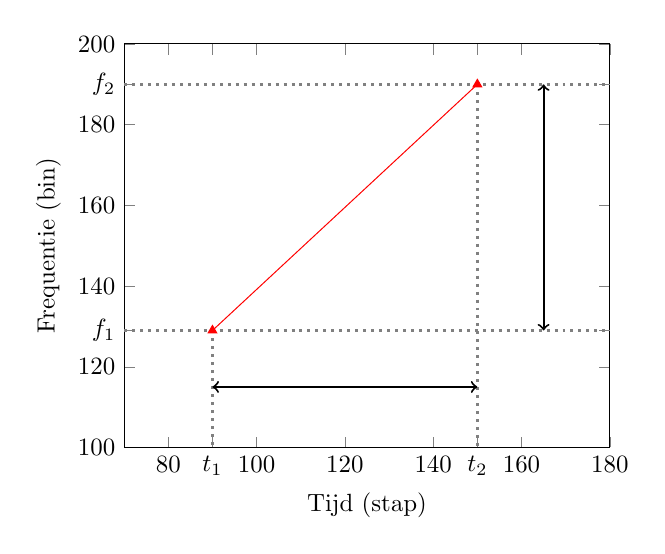
\begin{tikzpicture}[scale=0.9]
\begin{axis}[
	xlabel={Tijd (stap)},
	ylabel={Frequentie (bin)},
	xmin=70,xmax=180,
	ymin=100,ymax=200,
	legend style={
  		cells={anchor=west},
  		legend pos=outer north east,
	},
	extra y ticks={129,190}, 
	extra y tick labels={$f_1$,$f_2$},
	extra x ticks={90,150}, 
	extra x tick labels={$t_1$,$t_2$},
]

  % plot the data from the file data.dat
  % smooth the curve and mark the data point with a dot
  \addplot[color=red,mark=triangle*] coordinates {
  	(90,129)
  	(150,190)
  };
  
  %f1
   \addplot[style= dotted,color=gray,very thick] coordinates{ (70,129)
   (180,129)};
   %f2
   \addplot[style= dotted,color=gray,very thick] coordinates{ (70,190)
   (180,190)};
   
    \node at (99,60) [] {\small$\Delta f$};
    \addplot[color=black,<->,thick] coordinates{ (165,129) (165,190)};
    
   \node at (50,18) [] {\small$\Delta t$};
   \addplot[style=dotted,color=gray,very thick] coordinates{ (90,129)
   (90,100)}; 
   \addplot[style=dotted,color=gray,very thick] coordinates{
   (150,190) (150,100)};
   \addplot[color=black,<->,thick] coordinates{ (90,115)
   (150,115)};
  
  \end{axis}
\end{tikzpicture}
	\end{center}
\end{figure}

Na het extraheren en opslaan van de fingerprints kunnen er matches gezocht worden door de hashwaarden van de fingerprints van beide audiofragmenten met elkaar te vergelijken. Van elke match wordt de offset berekend, wat het verschil is tussen $ t1 $ van beide fingerprints. Wanneer beide fragmenten overeenkomen zal dit resulteren in een groot aantal matches met dezelfde offset. 

Accoustic fingerprinting kunnen we toepassen op streams door ze te bufferen. Na het opbouwen van de buffers dient het algoritme hierop te worden uitgevoerd. De maximale offset die gevonden werd bij het matchen komt overeen met de latency tussen beide streams.

Een uitgebreidere beschrijving is te vinden in artikel \cite{Wang2003a}. Deze methode is echter beperkt tot het vergelijken van audiofragmenten die in tijd noch toonhoogte gewijzigd zijn. Aan het IPEM is een aangepaste methode ontwikkeld die dit wel toelaat \cite{six2014panako}.

\subsubsection{Toepassing in realtime}

Door het bufferen van de streams kan accoustic fingerprinting gebruikt worden in een realtime toepassing. Afhankelijk van de gebruikte parameters en de kwaliteit van de audio is een buffergrootte van enkele seconden voldoende om de latency tussen de streams te bepalen. Verder in dit hoofdstuk zal het bufferen worden besproken.

De nauwkeurigheid van dit algoritme hangt af van de grootte van de \textit{FFT bins}. De waarde hiervan is afhankelijk van de parameters van het FFT algoritme. Een nauwkeurigheid van 16 ms of 32 ms is standaard.

\subsection{Kruiscovariantie}

Deze methode bepaalt de gelijkenis tussen twee audiofragmenten en resulteert in een bepaalde. De latency tussen twee audiofragmenten kan bepaald worden door deze berekening uit te voeren voor elke mogelijke verschuiving. De verschuiving waarbij de kruiscovariantie het hoogst is bepaalt de latency.

\subsubsection{Werking}

Stel twee audioblokken $ a $ en $ b $ bestaande uit $ s $ samples en verschuiving $ i $. Voor elke $ i $ gaande van 0 tot $ s $ wordt de kruiscovariantie berekent met volgende formule:

\begin{equation}
\sum_{j=0}^{s} a_{j} \cdot b_{(i+j)\ mod\ s}
\end{equation}

De waarde van $ i $ waarbij de kruiscovariantie het hoogst is stelt de latency voor tussen beide audioblokken in aantal samples. De latency in seconden bepaalt men door dit resultaat te delen door de samplefrequentie.

De methode kan de latency tot op één sample nauwkeurig bepalen. De maximaal bereikbare nauwkeurigheid hangt dus af van de samplefrequentie van de audioblokken. Bij een samplefrequentie van $8000 Hz$ is dit $ 1/8000 Hz = 0.125 ms $. Dit is ruim voldoende voor onze toepassing.

Een nadeel aan deze methode is de performantie. Het berekenen van de beste kruiscovariantie van twee audioblokken bestaande uit s samples kan gebeuren in  $O(s^{2})$. Het is dus belangrijk om bij deze berekening de grootte van de audioblokken te beperken.

In artikel \citealp{six2015multimodal} wordt deze techniek meer in detail besproken.

\subsubsection{Toepassing in realtime}

Het bufferen van de audiostreams maakt ook dit algoritme in realtime toepasbaar. In tegenstelling tot accoustic fingerprinting is het niet de bedoeling dat de berekeningen op de volledige buffer wordt uitgevoerd. Door de kwadratische tijdscomplexiteit zou dit onnoemelijk veel rekenkracht vragen.\footnote{Voor het berekenen van de kruiscovariantie tussen twee buffers met $10s$ audio en een samplefrequentie van $8000hz$ zijn er asymptotisch 6400000000 berekeningen vereist.} Hoe de berekening dan wel moet worden uitgevoerd wordt verderop uitgelegd.

\subsection{Toepasbaarheid}

Het accoustic fingerprinting algoritme is zeer snel en robuust en kan gebruikt worden om gebufferde audiostreams te synchroniseren tot enkele tientallen milliseconden nauwkeurig (afhankelijk van de parameters van het FFT algoritme).

Het kruiscovariantie algoritme kan eveneens gebruikt worden om (gebufferde) audiostreams te synchroniseren. De grootste troef van dit algoritme is haar nauwkeurigheid: in de beste omstandigheden kan het algoritme resultaten bekomen tot op één sample nauwkeurig. Het bereiken van een dergelijke nauwkeurigheid is onmogelijk met eender welk ander besproken algoritme. De keerzijde is de performantie van het algoritme. Bij het synchroniseren van grote audioblokken kan dit problematisch zijn.

De kenmerken van deze algoritmen zijn heel erg complementair. De gemakkelijkste manier om een robuust, snel én nauwkeurig systeem op te bouwen is door het beste van de twee werelden te combineren. Het accoustic fingerprinting algoritme kan zorgen voor de synchronisatie tot op enkele tientallen milliseconden nauwkeurig. Dit resultaat laat toe dat we het kruiscovariantie algoritme kunnen uitvoeren op zeer korte stukjes audio (een honderdtal milliseconden volstaat).

\section{Bufferen van streams}

\begin{figure}[h!]
	\captionsetup{width=0.7\textwidth}
	\caption[Schematische weergave van de buffer]{Schematische weergave van een verschuivende buffer over een audiostream.}
	\begin{center}
		\advance\parskip0.3cm
		\begin{tikzpicture}[scale=0.9]
\begin{axis}[
xlabel={Tijd (seconden)},
xmin=170,xmax=200,
ymin=0,ymax=1,
legend style={
	cells={anchor=west},
	legend pos=outer north east,
},
yticklabels={,,},
xticklabel style={grid=major},
extra x ticks={176,177,186,187},
extra x tick labels={,,,},
extra tick style={grid=major, grid style={dotted}},
hide y axis
]
\addplot[thick,black] graphics[xmin=140,ymin=0,xmax=200,ymax=1] {wave.png};

after end axis/.code={
	\draw[black,<->] (axis cs:175,0.1) -- (axis cs:185,0.1)	node [pos=0.5,above,font=\scriptsize] {buffer $i-1$};
	
	\draw[black,<->] (axis cs:176,0.2) -- (axis cs:186,0.2)	node [pos=0.5,above,font=\scriptsize] {buffer $i$};
	
	\draw[black,<->] (axis cs:177,0.3) -- (axis cs:187,0.3)	node [pos=0.5,above,font=\scriptsize] {buffer $i+1$};
}]

%\node at (50,18) [] {\small$\Delta t$};
%\addplot[style=dotted,color=gray,very thick] coordinates{ (90,129)
%	(90,100)}; 
%\addplot[style=dotted,color=gray,very thick] coordinates{
%	(150,190) (150,100)};
%\addplot[color=black,<->,thick] coordinates{ (90,115)
%	(150,115)};

\end{axis}

\end{tikzpicture}
	\end{center}
\end{figure}

Zowel in de introductie als bij de gedetailleerde bespreking van de algoritmes is er vaak aangehaald dat de streams gebufferd zullen worden. Hoe dit precies in zijn werk zal gaan is echter nog niet besproken. In dit deel wordt dit concept meer gedetaileerd uitgelegd.

Bij het bufferen maken we gebruik van een \textit{sliding window}. Deze techniek zorgt ervoor dat de algoritmes voldoende data hebben om berekeningen op uit te voeren terwijl wijzigingen aan de latency (door drift of gedropte samples) toch voldoende snel gedetecteerd worden.

De grootte van de buffer heeft invloed op de kwaliteit van de geretourneerde resultaten. Het is logisch dat de algoritmes de latency beter kunnen bepalen door 10s in plaats van 1s audio te analyseren. Een nadeel is echter dat het langer duurt vooraleer de latency of een wijziging ervan gedetecteerd kan worden. Indien er bijvoorbeeld buffers gebruikt worden die 10s audio kunnen bevatten, dan zal een wijziging aan de latency gemiddeld na iets meer dan 5 seconden gedetecteerd worden. Dit is te verklaren aangezien de buffer vanaf dat moment procentueel meer audio bevat met de gewijzigde latency dan audio met de oude latency.

In de evaluatiecriteria is er bepaald dat een wijziging aan de latency (door drift of gedropte samples) binnen één seconde gedetecteerd moet worden. Een verschuivende buffer kan hier voor zorgen: in plaats van een vast aantal seconden audio te bufferen en vervolgens de volledige grootte van de buffer op te schuiven wordt de buffer over een veel kleinere afstand verschoven. Hierdoor kunnen latencywijzigingen, ondanks de vertraging waarmee we de resultaten verkrijgen, toch nauwkeuriger en sneller bepaalt worden.

\chapter{Implementatie}

\section{Technologieën en software}

\subsection{Java 7}

Er zijn verschillende redenen waarom er gekozen is om de synchronisatie bibliotheek in Java te implementeren. De belangrijkste reden is dat de bestaande audio bibliotheken (Panako en TarsosDSP) van het IPEM ook ontwikkeld zijn in Java. Deze kunnen enkel aangeroepen worden via andere Java applicaties.

Het is ook de bedoeling is om de gebruikersinterface te ontwikkelen met behulp van Max/MSP modules. Het ontwikkelen van dergelijke modules is mogelijk in twee programmeertalen: C en Java. De eenvoud en hoge graad van abstractie gaf de doorslag om hierbij Java te gebruiken. De voordelen die C biedt op vlak van snelheid wegen (in deze toepassing) hier niet tegenop.

Hoewel de laatste versie van Max/MSP (7) het toelaat om Java 8 te gebruiken wordt deze versie in dit project om compatibiliteitsredenen vermeden. 



\subsection{TarsosDSP}

TarsosDSP is een Java bibliotheek voor realtime audio analyse en verwerking ontwikkeld aan het IPEM. De bibliotheek bevat een groot aantal algoritmes voor audioverwerking en kan nog verder worden uitgebreid. Deze bibliotheek wordt beschreven in artikel \cite{six2014tarsosdsp}. 

TarsosDSP is voornamelijk gebouwd rond het concept \textit{processing pipeline}. Dit is een abstractie van een audiostream die via programmacode verwerkt kan worden.  Een processing pipeline wordt voorgesteld als instantie van de klasse \texttt{AudioDispatcher}. Het aanmaken gebeurt met behulp van de klasse \texttt{AudioDispatcherFactory}. Deze bevat statische methodes om een \texttt{AudioDispatcher} aan te maken van een audiobestand, een array van floating-point getallen of een microfoon. Een processing pipeline kan bewerkt of verwerkt worden met behulp van één of meerdere \texttt{AudioProcessors}. Een \texttt{AudioProcessor} is een interface met de methodes \texttt{process} en \texttt{processingFinished}. De \texttt{process} methode heeft als enige parameter een \texttt{AudioEvent}. Dit object bevat een audio blok, voorgesteld als array van floating-point getallen met waarden tussen -1.0 en 1.0. De grootte van dit blokje audio, en de mate van overlapping tussen de opeenvolgende blokjes audio is instelbaar. Verder bevat dit object nog andere metadata zoals onder meer een \textit{timestamp}.

Afhankelijk van de implementatie van de \texttt{process} methode kan de audiostroom op een bepaalde manier verwerkt, geanalyseerd of gewijzigd worden.

TarsosDSP bevat verder nog een groot aantal klassen met allerhande tools en audioverwerkings algoritmen. Het merendeel hiervan maakt gebruik van de zojuist beschreven processing pipeline. 

Een greep uit de features van TarsosDSP:
\begin{itemize}[noitemsep]
	\item Toevoegen van geluidseffecten (delay, flanger,...)
	\item Toevoegen van filters (low-pass, high-pass, band-pass,...)
	\item Conversie tussen verschillende formaten
	\item Toonhoogte detectie
	\item Wijzigen van de samplefrequentie
	\item FFT analyse
\end{itemize}

\subsection{Panako}

Panako is net zoals TarsosDSP een Java bibliotheek (door de zelfde auteur) ontwikkeld aan het IPEM. Panako bevat een arsenaal aan algoritmen voor het matchen of synchroniseren van audiofragmenten of audiostreams.  Deze bibliotheek wordt uitgebreid beschreven in artikel \cite{six2014panako}.

In dit onderzoek wordt vooral gebruik gemaakt van Panako's open-source implementatie van het accoustic fingerprinting algoritme. Dit algoritme wordt beschreven in de paper van Avery Li-Chun Wang\cite{Wang2003a}. Het algoritme uit de paper is verder uitgebreid zodat audio waarbij de toonhoogte verhoogd of verlaagd is, of audio die sneller of trager is afgespeeld, toch gedetecteerd kan worden.

Buiten het eigenlijke algoritme bevat de bibliotheek ook verschillende toepassingen die hiervan gebruik maken. Zo is het mogelijk om de fingerprints van een geluidsfragment te bekijken, matches tussen verschillende geluidsfragmenten te visualiseren, en grafisch te experimenteren met de verschillende parameters. Figuur \ref{fingerprint_visualiser} toont een screenshot van deze toepassing.

\begin{figure}[!h]
	\captionsetup{width=0.8\textwidth}
	\caption[Gebruikersinterface van Audacity]{De gebruikersinterface van Panako's NFFT Fingerprint Visualiser. Onderaan kunnen de parameters van het algoritme met behulp van sliders gewijzigd worden.}
	\centering
	\advance\parskip0.3cm
	\includegraphics[width=0.8\textwidth]{fingerprint_visualiser.png}
	\label{fingerprint_visualiser}
\end{figure}

Er is ook een applicatie beschikbaar om verschillende geluidsfragmenten te synchroniseren. Deze applicatie maakt behalve van het accoustic fingerprinting algoritme ook nog gebruik van het kruiscovariantie algoritme. 

Wanneer de latency tussen de verschillende audiofragmenten bepaald is, dan kan de applicatie een shell script genereren dat met behulp van \textit{FFmpeg} stukjes van de geluidsbestanden wegknipt of er stilte aan toevoegt. Het resultaat is dat na het uitvoeren van het script de geluidsbestanden gesynchroniseerd zijn.

\subsection{FFmpeg}

FFmpeg is een command-line multimedia framework dat gebruikt wordt voor encoderen, decoderen, multiplexen, demultiplexen, streamen en afspelen van audio en video. \cite{kollarconfiguration}

In dit onderzoek wordt FFmpeg voornamelijk gebruikt in scripts bij het geautomatiseerd genereren van testdata.

\subsection{SoX}

SoX is net zoals FFmeg een command-line tool voor audioverwerking. Buiten de mogelijkheid om audiobestanden te converteren laat SoX ook minder triviale operaties toe. Zo is het onder meer mogelijk om het volume aan te passen, effecten toe te voegen, de bestanden bij te knippen of gegenereerde geluiden in een audiobestand te mixen.
\cite{barras2012sox}

In dit onderzoek wordt SoX ook gebruikt in scripts bij het manipuleren van de testdata.

\subsection{Sonic Visualiser}

Sonic Visualiser is een gebruiksvriendelijke desktopapplicatie voor de analyse, visualisatie van audiobestanden. Sonic Visualiser laat toe om audiobestanden vanuit verschillende perspectieven te analyseren, zo kan zowel de waveform als het spectrogram van een audiobestand gevisualiseerd worden. Sonic Visualiser is uitbreidbaar met plug-ins in het Vamp formaat. \cite{cannam2010sonic}

\begin{figure}[!h]
	\captionsetup{width=0.8\textwidth}
	\caption[Gebruikersinterface van Sonic Visualiser]{De gebruikersinterface van Sonic Visualiser}
	\advance\parskip0.3cm
	\centering
	\includegraphics[width=0.8\textwidth]{sonicvisualiser.png}
\end{figure}

Sonic Visualiser werd in dit onderzoek vooral gebruikt om handmatig de latency tussen verschillende audiofragmenten te bepalen. Ook heeft de applicatie dienst gedaan als educatieve tool om verschillende audioverwerkingsalgoritmen visueel voor te stellen.
\vspace{0.5cm}

\subsection{Audacity}

Audacity is een open-source desktopapplicatie voor het bewerken, opnemen en converteren van audio. Met Audacity is het ook mogelijk om tal van effecten en filters aan audio toe te voegen.\cite{audacity2016}

\begin{figure}[!h]
	\captionsetup{width=0.8\textwidth}
	\caption[Gebruikersinterface van Audacity]{De gebruikersinterface van Audacity}
	\centering
	\advance\parskip0.3cm
	\includegraphics[width=0.8\textwidth]{audacity.png}
	\label{screenshot-audacity}
\end{figure}

Alle opnames en handmatige bewerkingen op audiobestanden in dit onderzoek zijn uitgevoerd met behulp van Audacity. 

Figuur \ref{screenshot-audacity} toont de gebruikersinterface van dit programma.

\subsection{Max/MSP}

Max/MSP is een visuele programmeertaal voor muziek en multimedia. Het is een systeem waarbij modules met elkaar verbonden kunnen worden om zo complexere systemen op te bouwen. Max/MSP beschikt ook over een API waarmee in Java of C nieuwe modules ontwikkeld kunnen worden. \cite{cycling2016}

\begin{figure}[!h]
	\captionsetup{width=0.8\textwidth}
	\caption[Gebruikersinterface van MAX/MSP]{De gebruikersinterface van Max/MSP: een \textit{patch panel} met daarop enkele modules die samen een complexere toepassing vormen.}
	\centering
	\advance\parskip0.3cm
	\includegraphics[width=0.8\textwidth]{maxmsp.png}
	\label{screenshot-max}
\end{figure}

Met Max/MSP is het mogelijk om realtime audio verwerken, daarom zal deze toepassing gebruikt worden voor het ontwikkelen van de gebruikersinterface. 

Figuur \ref{screenshot-max} toont hoe een eenvoudige Max/MSP patch er grafisch uitziet.

\subsection{Teensy}

De Teensy is een kleine microcontroller die via USB geprogrammeerd kan worden. De Teensy is compatibel met de Arduino software en is hierdoor zeer gebruiksvriendelijk. \cite{teensy2016}

De sensoren die gebruikt worden bij de experimenten van het IPEM zijn meestal aangesloten op Teensy microcontrollers.
Om de synchronisatiealgoritmes en het bijhorende systeem in een representatieve situatie te testen zal daarom ook gebruik gemaakt worden van een Teensy microcontroller.

\begin{figure}[!h]
	\captionsetup{width=0.7\textwidth}
	\caption[Teensy microcontroller]{De Teensy microcontroller verbonden met een infraroodsensor en microfoon op een breadboard.}
	\centering
	\advance\parskip0.3cm
	\includegraphics[width=0.4\textwidth]{teensy.jpg}
	\label{teensy-pic}
\end{figure}

In hoofdstuk \ref{evaluatie} wordt de testen die met de Teensy microcontroller zijn uitgevoerd meer in detail besproken. Figuur \ref{teensy-pic} toont een typische testopstelling waarbij twee sensoren zijn aangesloten op de microcontroller.

\section{Accoustic fingerprinting}

De Panako softwarebibliotheek bevat een implementatie van het accoustic fingerprinting algoritme. Om wijzigingen mogelijk te maken hebben is de code van het algoritme overgenomen in het project van dit onderzoek. De overgenomen code blijft wel nog steeds afhankelijk van enkele klassen uit het Panako project. 

\subsection{Optimalisaties}

Aan dit algoritme is één vereenvoudiging aangebracht. Het originele algoritme bevatte namelijk de mogelijkheid om alle offsets boven een bepaalde drempelwaarde te verwerken. Deze feature laat toe dat er meerdere matches kunnen gevonden worden binnen één uitvoering van het algoritme. Om dit te ondersteunen moeten alle matches echter wel één voor één worden vergeleken met de drempelwaarde. Omdat we in dit onderzoek enkel geïnteresseerd zijn in de beste offsetwaarde is dit overbodig. De beste offset en bijhorende fingerprints wordt apart bijgehouden. De naverwerking wordt hierdoor vermeden.

\subsection{Parameters en hun invloed op het algoritme}
\label{accoustic-fingerprinting-params}

De werking van dit algoritme is afhankelijk van een aantal parameters die een grote invloed kunnen hebben op de performantie en de nauwkeurigheid van het uiteindelijke resultaat. Daarom is het van belang om voor het uitvoeren van het algoritme de waarde van deze parameters te controleren. De optimale waarde van elke parameter is afhankelijk van verschillende factoren die van situatie tot situatie kunnen verschillen:

\begin{itemize}[noitemsep]
\item de vereiste nauwkeurigheid van het algoritme;
\item de vereiste performantie van het algoritme;
\item de mate waarin er omgevingsgeluid aanwezig is;
\item de opnamekwaliteit van het omgevingsgeluid.
\end{itemize}

De meeste parameters worden bijgehouden in een configuratiebestand waardoor ze ook na compilatie wijzigbaar zijn. Dit zijn de belangrijkste parameters uit het configuratiebestand die invloed hebben op het algoritme:

\begin{description}
\item\texttt{SAMPLE\_RATE} \hfill \\
Deze parameter bepaalt de standaard samplefrequentie die gebruikt wordt tijdens het synchronisatieproces. Het verhogen van deze parameter zorgt voor een tragere verwerking maar een betere nauwkeurigheid. Afhankelijk van op welke manier de synchronisatie wordt opgestart (via Max of met een \texttt{AudioDispatcher}) worden de binnenkomende streams geresamplet of wordt al een correcte samplefrequentie verondersteld.

\item\texttt{NFFT\_BUFFER\_SIZE}\footnote{De letter N in NFFT heeft geen noemenswaardige betekenis. De naam is overgenomen van de gelijknamige parameter uit de Panako bibliotheek.} \hfill \\
Dit is de grootte van de verschuivende buffer die gebruikt wordt in het FFT algoritme. Deze parameter is cruciaal aangezien de frequentiesterktes op een bepaalde plaats op de tijd\-as worden berekend per buffer. Deze parameter wordt uitgedrukt in aantal samples.
\item\texttt{NFFT\_STEP\_SIZE} \hfill \\
Dit is het aantal samples elke verschuiving in het FFT algoritme. De stepsize beïnvloedt rechtstreeks de nauwkeurigheid van het accoustic fingerprinting algoritme. Wanneer deze parameter is ingesteld op 128 samples en een samplefrequentie van 8000hz dan is de maximale nauwkeurigheid $128/8000Hz = 0.016s = 16ms$.
\item\texttt{MIN\_ALIGNED\_MATCHES} \hfill \\
Een match tussen twee audiofragmenten wordt pas als geldig beschouwd wanneer er een bepaald aantal fingerprint matches met dezelfde offset gevonden zijn. Dit aantal wordt ingesteld met deze parameter.
\item\texttt{NFFT\_MAX\_FINGERPRINTS\_PER\_EVENT\_POINT} \hfill \\
Deze parameter bepaalt het maximum aantal fingerprints waaraan een event point (een punt op het spectrogram) kan deelnemen. Hoe hoger dit maximum hoe vlugger er matches kunnen gevonden worden. Bij een hoge waarde moeten meer berekeningen worden uitgevoerd, dit heeft invloed op de performantie.
\item\texttt{NFFT\_EVENT\_POINT\_MIN\_DISTANCE} \hfill \\
Dit is de minimale afstand tussen twee event points op het spectrogram die samen een fingerprint kunnen vormen. 

\end{description}

Verder maakt het algoritme nog gebruik van twee hardgecodeerde parameters die niet instelbaar zijn via het configuratiebestand: \texttt{MIN\_FREQUENCY} en \texttt{MAX\_FREQUENCY}. Deze parameters bepalen binnen welke frequentiebereik er naar fingerprints gezocht worden. De waarden waarop deze ingesteld staan bevinden zich op de rand van de frequenties die door muziek of stemgeluid geproduceerd worden.

\subsection{Optimale instellingen}
\label{optimal-accoustic-fingerprinting}

Het bepalen van de optimale waarden voor de parameters is geen exacte wetenschap maar eerder een probleem dat proefondervindelijk moet worden aangepakt.

Bij het accoustic fingerprinting algoritme is er een groot verschil tussen de meest ``elegante'' parameterwaarden en de in de praktisch presterende waarden. Dit verschil zal duidelijk worden in volgende opsomming waarin elke parameter zal worden besproken.


\begin{description}
	\item\texttt{SAMPLE\_RATE} \hfill \\
	Bij deze parameter is het van belang om een goede balans te vinden zodat de geluidskwaliteit aanvaardbaar blijft zonder een hypotheek te plaatsen op de performantie van het algoritme. De praktijk heeft uitgewezen dat bij een samplefrequentie van $ 8000Hz $ het algoritme goed presteert. Deze waarde wordt bevestigd in artikel \cite{six2015multimodal}.
	\item\texttt{NFFT\_BUFFER\_SIZE} en \texttt{NFFT\_STEP\_SIZE} \hfill \\
	De ingesteld waarden van de samplefrequentie, buffergrootte en stapgrootte zijn afhankelijk van elkaar. Om een goede werking van het FFT algoritme te garanderen bij een samplefrequentie van $ 8000Hz $ worden de buffergrootte en stapgrootte respectievelijk ingesteld op 512 en 128 (of 256) samples. Deze waarden worden eveneens vermeld in artikel \cite{six2015multimodal}.
	\item\texttt{MIN\_ALIGNED\_MATCHES} \hfill \\
	In een toepassing zoals het detecteren van liedjes ten opzichte van een database is het secuur instellen van deze parameter erg belangrijk. Deze parameter heeft namelijk een grote invloed op het voorkomen van \textit{false positives} of \textit{false negatives}. 
	
	Bij het synchroniseren van streams is de situatie echter helemaal anders. Het binnenkrijgen van een false positive (=foute latency) is veel minder erg dan het helemaal niet binnenkrijgen van (mogelijk correcte) resultaten. Aangezien het algoritme per buffer enkel het beste resultaat teruggeeft is de kans dat bij geluidsfragmenten van behoorlijke kwaliteit eenzelfde foute latency meer voorkomt dan de correcte latency zéér klein.
	
	Bij geluidsfragmenten van mindere kwaliteit kan het gebeuren dat er toch foute resultaten door de mazen van het net glippen. Om dit te vermijden is het mogelijk om nog een extra filtering toe te passen. In deze extra stap worden eventuele uitschieters geëlimineerd.
	
	Bovenstaande argumenten stellen duidelijk dat het beter is om deze parameter een lage waarde te geven. In deze toepassing is gekozen voor de waarde 2 in plaats van het absolute minimum 1: hierdoor wordt pure willekeur bij het matchen van audiofragmenten van extreem slechte kwaliteit vermeden.
	
	\item\texttt{NFFT\_MAX\_FINGERPRINTS\_PER\_EVENT\_POINT} \hfill \\
	In Panako is het standaard dat een event point uitmaakt van maximaal 2 fingerprints. Het hanteren van deze waarde leidt ertoe dat het matchen van audiofragmenten van behoorlijke kwaliteit zeer snel kan worden uitgevoerd. 
	
	In deze toepassing is het aantal te vergelijken audiofragmenten meestal erg beperkt. Ook is de kwaliteit van deze fragmenten vaak van ondermaats (bv. de opnames op microcontrollers). Daarom is het in dit geval een goed idee om de waarde van deze parameter zéér hoog in te stellen. Hierdoor verhoogt de kans sterk dat er bij zeer slechte audiofragmenten toch enkele overeenkomende fingerprints gevonden worden. Testen hebben uitgewezen dat de negatieve invloed op de performantie beperkt blijft en dat de resultaten sterk verbeteren. 
	
	Bij het zoeken naar matches tussen geluidsopnames opgenomen op microcontrollers heeft de praktijk uitgewezen dat het toelaten van maximaal 50 fingerprints per event point degelijke resultaten oplevert.
	%TODO: refereren naar testresultaen
	
	\item\texttt{NFFT\_EVENT\_POINT\_MIN\_DISTANCE} \hfill \\
	In tegenstelling tot vorige parameter zorgt het verhogen van deze waarde ervoor dat er minder fingerprints worden gecreëerd. De argumenten die bij vorige parameter zijn aangehaald gelden bijgevolg in omgekeerde zin ook voor deze parameter. Hoewel de Panako standaard 600 is leveren waardes rond het getal 20 in deze toepassing de beste resultaten zonder de performantie sterk te beperken.
	
	
\end{description}


\section{Kruiscovariantie}

De Panako bibliotheek bevatte bij aanvang van dit onderzoek ook al een implementatie van het kruiscovariantie algoritme. In tegenstelling tot het accoustic fingerprinting algoritme was het echter minder grondig afgewerkt. Om degelijke resultaten te garanderen was het noodzakelijk om enkele anomalieën in de geleverde resultaten te analyseren en de oorzaak hiervan op te lossen.

Net zoals het accoustic fingerprinting algoritme is de code overgenomen in het project van dit onderzoek. De code is echter niet meer afhankelijk van de Panako bibliotheek.

\subsection{Integratie met accoustic fingerprinting}
\label{integratie-accoustic-fingerprinting}

In sectie \ref{toepasbaarheid} is vermeld dat de latency eerst ruw berekend wordt met accoustic fingerprinting. Dit resultaat wordt vervolgens verfijnd door de kruiscovariantie tussen de signalen te berekenen. De werking hiervan zal verduidelijkt worden met behulp van een voorbeeld.

Onderstel twee geluidsopnames: de tweede opname heeft een vertraging van 90 ms ten opzichte van de eerste referentieopname. Het uitvoeren van het accoustic fingerprinting algoritme met standaard parameters (tot op $ 32 ms $ nauwkeurig) kan twee resultaten opleveren: $ 64 ms $ of $ 96 ms $.\footnote{Mogelijke resultaten: $ 2 \cdot 32 ms = 64 ms$ of $ 3 \cdot 32 ms = 96 ms $. De absolute fout is  met een waarde van $ 6 ms $ bij een latency van $ 96 ms $ het kleinst in vergelijking met $ 26 ms $ bij een latency van $ 64 ms $. Daarom is de kans het grootst dat $ 96 ms $ als resultaat zal worden teruggegeven.} Bij het eerste resultaat wordt de werkelijke latency onderschat. De tweede latency overschat deze waarde. Na het berekenen van de kruiscovariantie is dit van belang om het resultaat correct te verfijnen. In figuur \ref{crosscovariance1} worden de situatie visueel verduidelijkt.

\begin{figure}[h!]
	\captionsetup{width=0.7\textwidth}
	\caption[Kruiscovariantie audiofragmenten]{Twee audiofragmenten: het tweede audiofragment heeft een latency van 90 milliseconden ten opzichte van het eerste.}
	\begin{center}
		\advance\parskip0.3cm
		\begin{tikzpicture}[scale=1]
\begin{axis}[
xlabel={Tijd (milliseconden)},
xmin=0,xmax=500,
ymin=0,ymax=1,
legend style={
	cells={anchor=west},
	legend pos=outer north east,
},
yticklabels={,,},
xticklabel style={grid=major},
extra x ticks ={64,90,96},
extra x tick labels={,,,},
extra tick style={grid=major, grid style={dotted}},
hide y axis
]

\addplot[thick,black] graphics[xmin=0,ymin=0.5,xmax=500,ymax=0.8] {reference.png};

\addplot[thick,black] graphics[xmin=0,ymin=0.0,xmax=500,ymax=0.3] {other.png};


after end axis/.code={

	
	\draw[black,<->] (axis cs:0,0.42) -- (axis cs:96,0.42)	node [pos=0.5,above,font=\scriptsize] {$96ms$};
	
	\draw[black,<->] (axis cs:0,0.32) -- (axis cs:90,0.32)	node [pos=0.5,above,font=\scriptsize] {$90ms$};
	
	\draw[black,<->] (axis cs:0,0.22) -- (axis cs:64,0.22)	node [pos=0.5,above,font=\scriptsize] {$64ms$};
}]

\node at (axis cs:250,0.82) [] {Referentie};
\node at (axis cs:250,0.35) [] {Andere};

\end{axis}

\end{tikzpicture}
	\end{center}
	\label{crosscovariance1}
\end{figure}

Na het uitvoeren van het accoustic fingerprinting algoritme wordt er van beide fragmenten een blokje audio weggeknipt afhankelijk van de ruw bepaalde latency. Na deze stap is de latency van het resterende audiofragment zeker minder dan de minimale nauwkeurigheid van het accoustic fingerprinting algoritme. Vervolgens wordt het begin van elk audiofragment gekopieerd naar een buffer van een honderdtal samples. Daaropvolgend wordt de latency tussen deze twee buffers berekend met de kruiscovariantie methode. Deze latency is echter nog niet de latency waarnaar er uiteindelijk gezocht wordt. Er is nog een extra stap vereist waarbij de latency van het accoustic fingerprinting algoritme gecombineerd wordt met de latency van het kruiscovariantie algoritme. Figuur \ref{crosscovariance2} toont de buffers waarop het algoritme kan worden uitgevoerd. Elke buffer bevat 512 samples ($ 64 ms $ bij een samplefrequentie van $ 8000 Hz $).

\begin{figure}[h!]
	\captionsetup{width=0.7\textwidth}
	\caption[Kruiscovariantie buffers]{Kruiscovariantie buffers na het wegknippen van de $ 96 ms $ latency bepaald door het accoustic fingerprinting algoritme. Hier heeft de referentie audio $ 6 ms $ latency ten opzichte van het andere audiofragment.   }
	\begin{center}
		\advance\parskip0.3cm
		\begin{tikzpicture}[scale=1]
\begin{axis}[
xlabel={Tijd (milliseconden)},
xmin=0,xmax=64,
ymin=0,ymax=1,
legend style={
	cells={anchor=west},
	legend pos=outer north east,
},
yticklabels={,,},
xticklabel style={grid=major},
%extra x ticks ={64,90,96},
extra x tick labels={,,,},
extra tick style={grid=major, grid style={dotted}},
hide y axis,
width = 15cm,
height = 7cm
]

\addplot[thick,black] graphics[xmin=0,ymin=0.6,xmax=64,ymax=0.9] {refcut.png};

\addplot[thick,black] graphics[xmin=0,ymin=0.1,xmax=64,ymax=0.4] {othercut.png};


after end axis/.code={
	\draw[black,<->] (axis cs:0,0.85) -- (axis cs:6,0.85)	node [pos=0.5,above,font=\scriptsize] {$6ms$};
}]

\node at (axis cs:32,0.85) [] {Referentie};
\node at (axis cs:32,0.37) [] {Andere};

\end{axis}

\end{tikzpicture}
	\end{center}
	\label{crosscovariance2}
\end{figure}

Intuïtief lijkt het logisch dat deze latencies enkel bij elkaar moeten worden opgeteld om de verfijnde latency te bekomen. Toch is dit niet helemaal correct. Wanneer het accoustic fingerprinting algoritme de werkelijke latency heeft onderschat levert deze optelling een correct resultaat. Bij een overschatting is dit echter niet het geval. Dit probleem is duidelijk zichtbaar in figuur \ref{crosscovariance2}: na het wegknippen van de ruwe latency ($96 ms$) is de latency omgedraaid: de referentie audio heeft $ 6 ms $ latency ten opzichte van het andere audiofragment. 

Aangezien het kruiscovariantie algoritme de latency zoekt van de ``andere'' buffer ten opzichte van de referentiebuffer zal het resultaat niet $6 ms$ maar $ 58 ms $ zijn. Dit komt doordat het algoritme de ``andere'' buffer cyclisch (maar in de verkeerde zin) verschuift. Een verschuiving van $ 58 ms $ is bijgevolg de meest optimale verschuiving.

Om in een dergelijke situatie de verfijnde latency te berekenen moet men de latency verkregen door het kruiscovariantie algoritme ($ 58 ms$) aftrekken van de lengte van de gebruikte buffer ($ 64 ms $). De verfijnde latency bekomt men vervolgens door dit resultaat ($ 6 ms $) af te trekken van de latency van het fingerprinting  algoritme ($ 96 ms - 6 ms = 90 ms $).

%Eventueel nog schrijven hoe bepaald wordt of het resultaat onderschat of overschat is.

\subsection{Optimalisaties}

\subsubsection{Bugfixes}

In de originele versie van het algoritme werd er geen rekening gehouden met het feit dat het accoustic fingerprinting algoritme het de werkelijke latency kan overschatten of onderschatten. De latency bepaalt door het kruiscovariantie algoritme werd telkens opgeteld bij de ruwe latency bepaald door het accoustic fingerprinting algoritme. In 50\% van de gevallen leidde dit probleem tot foutieve resultaten.

\subsubsection{Meerdere malen uitvoeren van het algoritme}

In tegenstelling tot accoustic fingerprinting is het bepalen van de latency met kruiscovariantie veel meer foutgevoelig. Bij opnames van slechte kwaliteit worden vaak foute resultaten teruggegeven. 

Hoewel bij accoustic fingerprinting mogelijk storende factoren (een zoemende toon, geruis,...) zichtbaar zijn in het spectrogram zullen er naar alle waarschijnlijkheid nog steeds voldoende fingerprints gegenereerd worden op basis van geluiden die wel in beide opnames voorkomen. 

\begin{figure}[h!]
	\captionsetup{width=0.7\textwidth}
	\caption[Zoemtoon van $50 Hz$]{Twee gelijke audiofragmenten. Aan het tweede audiofragment is een achtergrondtoon van $50 Hz$ toegevoegd.}
	\begin{center}
		\advance\parskip0.3cm
		\begin{tikzpicture}[scale=1]
\begin{axis}[
xlabel={Tijd (milliseconden)},
xmin=0,xmax=140,
ymin=0,ymax=1,
legend style={
	cells={anchor=west},
	legend pos=outer north east,
},
yticklabels={,,},
xticklabel style={grid=none},
extra x tick labels={,,,},
extra tick style={grid=major, grid style={dotted}},
hide y axis,
width = 15cm,
height = 6cm
]

\addplot[thick,black] graphics[xmin=0,ymin=0.6,xmax=140,ymax=0.9] {zoemtoon-origineel.png};

\addplot[thick,black] graphics[xmin=0,ymin=0.1,xmax=140,ymax=0.4] {zoemtoon.png};


after end axis/.code={
%	\draw[black,<->] (axis cs:0,0.85) -- (axis cs:6,0.85)	node [pos=0.5,above,font=\scriptsize] {$6ms$};
}]

\node at (axis cs:70,0.88) [] {Origineel fragment};
\node at (axis cs:70,0.40) [] {Fragment met $50 Hz$ toon};

\end{axis}

\end{tikzpicture}
	\end{center}
	\label{zoemtoon}
\end{figure}

Dergelijke storende elementen hebben veel meer invloed op het kruiscovariantie algoritme. Een ongewenste zoemende bastoon zorgt voor een grote verandering van de geluidsgolf van het audiofragment. Aangezien de kruiscovariantie rechtstreeks tussen twee geluidsgolven berekent wordt kan dit serieuze gevolgen hebben. In figuur \ref{zoemtoon} wordt dit probleem visueel verduidelijkt.

De invloed van storende factoren zoals zoemende tonen en ruis is gemakkelijk te beperken. Aangezien het kruiscovariantie algoritme over een zéér klein deeltje van het audiofragment wordt uitgevoerd is het zeer eenvoudig om het algoritme tientallen keren, maar telkens op een andere plaats, uit te voeren. Na elke iteratie wordt de latency in het geheugen opgeslagen. Ten slotte wordt er gezocht naar de latency die het meeste voorkomt. Die latency wordt gebruikt om het resultaat van het accoustic fingerprinting algoritme te verfijnen.

\subsection{Parameters en hun invloed op het algoritme}

De parameters van het kruiscovariantie algoritme zijn net zoals die van het accoustic fingerprinting algoritme instelbaar via het configuratiebestand.

\begin{description}	
	\item\texttt{NFFT\_BUFFER\_SIZE} \hfill \\
	Hoewel het FFT algoritme eigenlijk niets te maken heeft met het berekenen van de kruiscovariantie speelt deze parameter bij dit algoritme toch een belangrijk rol. Deze parameter bepaalt namelijk de grootte van de buffers waartussen de kruiscovariantie berekent wordt. Om een goede werking van het kruiscovariantie algoritme te verzekeren is het een vereiste dat de gebruikte buffers groter zijn dan de minimale nauwkeurigheid van het accoustic fingerprinting algoritme (anders is het mogelijk dat na het knippen de audiofragmenten er geen gelijkenissen te vinden zijn tussen beide buffers). Aangezien deze nauwkeurigheid bepaald wordt de \texttt{NFFT\_STEP\_SIZE} parameter en de \texttt{NFFT\_BUFFER\_SIZE} hier altijd een veelvoud van is, is het gemakkelijk om deze parameter ook voor het kruiscovariantie algoritme te gebruiken.
	
	\item\texttt{CROSS\_COVARIANCE\_NUMBER\_OF\_TESTS} \hfill \\
	Deze parameter bepaalt het aantal keren dat het kruiscovariantie algoritme per streambuffer (zie \ref{streambuffers}) zal worden uitgevoerd. De meest voorkomende latency wordt als resultaat teruggegeven.
	
	\item\texttt{CROSS\_COVARIANCE\_THRESHOLD} \hfill \\
	Deze parameter bepaalt het minimum aantal keer dat een latency moet voorkomen om als geldig beschouwt te mogen worden.	Stel dat het algoritme 50 keer wordt uitgevoerd maar elke keer een verschillend resultaat teruggeeft, dan zal er geen latency worden teruggegeven indien deze parameter staat ingesteld op een waarde groter dan 1.
	
\end{description}

\subsection{Optimale instellingen}
\begin{description}	
	\item\texttt{NFFT\_BUFFER\_SIZE} \hfill \\
	De optimale waarde van deze parameter werd in sectie \ref{optimal-accoustic-fingerprinting} besproken.
	
	\item\texttt{CROSS\_COVARIANCE\_NUMBER\_OF\_TESTS} \hfill \\
	Bij audiofragmenten van goede kwaliteit is het niet noodzakelijk om deze parameter een hoge waarde te geven. Als het algoritme 5 à 10 keer wordt uitgevoerd zal de correcte latency hoogst waarschijnlijk al verschillende malen gevonden zijn. 
	
	Bij audiofragmenten van slechte kwaliteit is het van belang om deze parameter zo hoog mogelijk in te stellen. Aangezien het kruiscovariantie algoritme vrij intensief is hangt de waarde wat af van de beschikbare rekenkracht. De praktijk heeft uitgewezen dat de waarde 50 een goed evenwicht biedt tussen correctheid en performantie.
	
	Dit aantal heeft als bovengrens ($ N_B $) het aantal keren dat een kruiscovariantie buffer (bepaald door \texttt{NFFT\_BUFFER\_SIZE}) past in een streambuffer (zie \ref{streambuffers}) waarin de streams worden ingelezen (bepaald door \texttt{SLICE\_SIZE\_S}). Dit kan worden berekend met volgende formule:
	\begin{equation}
		N_B = \frac{\texttt{SLICE\_SIZE\_S}}{\texttt{NFFT\_BUFFER\_SIZE} \cdot \texttt{SAMPLE\_RATE}}
	\end{equation}
	
	\item\texttt{CROSS\_COVARIANCE\_THRESHOLD} \hfill \\
	Het hoog instellen van deze waarde heeft enkel nut als het van belang is dat het kruiscovariantie algoritme zeker een correct resultaat teruggeeft. In de huidige implementatie wordt het ruwe resultaat gebruikt als6 het aantal gelijke waarden niet boven deze drempel komt. Daarom wordt deze waarde meestal op 1 ingesteld. De best mogelijke verfijning van het resultaat wordt dan toegepast, ongeacht het aantal keer dat het resultaat voorkomt. 
\end{description}

\section{Filteren van de resultaten}
\label{filtering}

Het is moeilijk om met zekerheid te bepalen of een bepaalde latency correct is. Toch kan er een soort van statistische optimalisatie worden uitgevoerd op de opeenvolgende latencies. De kans is namelijk klein dat de werkelijke latency verandert en na een korte tijd terugkeert naar de originele waarde.\footnote{Theoretisch is een dergelijke situatie toch mogelijk: In dit voorbeeld wordt de latency bepaalt tussen de audiostreams ($ 8000 Hz$ samplefrequentie) van twee Teensy microcontrollers. Wanneer er 50 samples gedropt worden van de referentie audiostream zorgt dit voor een latencyverhoging van de andere audiostream van $6 ms$. Indien er enkele seconden later 50 samples gedropt worden van de andere audiostream dan leidt dit tot een vermindering van de latency van $ 6 ms $. Visueel is dit een piek in de opeenvolgende latencies.} Ook is de kans klein dat een foute latency toevallig verschillende malen na elkaar gedetecteerd wordt.

Deze eigenschappen laten toe om toch een bepaalde vorm van ``foutherstelling'' te implementeren. Fouten kunnen namelijk weggefilterd worden door eventuele pieken in opeenvolgende latencies af te vlakken.

\subsection{Werking}

Het afvlakken van pieken kan in realtime geïmplementeerd worden door opnieuw gebruik te maken van verschillende \textit{sliding windows}. Per audiostream wordt een buffer bijgehouden met daarin de opeenvolgende latencies ten opzichte van de referentie audiostream. Wanneer een buffer haar maximumcapaciteit heeft bereikt gaat het toevoegen van een nieuwe latency gepaard met het verwijderen van de oudste latency.

Het afvlakken van pieken wordt verwezenlijkt door in plaats van de meest recente latency het gemiddelde of de mediaan van de buffer te gebruiken. De mate waarin pieken worden afgevlakt hangt af van de grootte van de buffer en de gebruikte methode (gemiddelde of mediaan).

\subsection{Voorbeelden}

De effectiviteit van de verschillende parameters (buffergrootte en filtermethode) zal in dit gedeelte worden weergegeven aan de hand van enkele voorbeelden. Er zullen verschillende soorten filters worden toegepast op een verloop van 35 latencies. In het ongefilterde verloop (zie figuur \ref{latencydata}) komen twee grote en drie kleine pieken voor. Na het vijftiende resultaat doet er zich een blijvende verhoging van de latency voor.

\begin{figure}[h!]
	\captionsetup{width=0.7\textwidth}
	\caption[Het ongefilterde verloop van de latency]{Grafische weergave van het ongefilterde verloop van de latency.}
	\begin{center}
		\advance\parskip0.3cm
		\input{figuren/latencydata}
	\end{center}
	\label{latencydata}
\end{figure}

\subsubsection{Moving average filter}

De eerste twee voorbeelden tonen het verschil tussen de ongefilterde latencies en de latencies die gefilterd zijn door het gemiddelde van een buffer te nemen. Bij het eerste voorbeeld bevat de buffer maximum 3 latencies, bij het tweede voorbeeld kan de buffer maximum 5 latencies bevatten.

\begin{figure}[!tbph]
	\centering
	\subfloat[Buffergrootte 3]{\begin{tikzpicture}[scale=0.9]
\begin{axis}[
ylabel={Latency (ms)},
xtick ={0,5,10,15,...,35},
ytick ={60,80,...,180},
ymin = 60,
ymax = 180,
height = 5cm,
width = 8cm
]
\addplot [mark=none] table {avg3data.dat};
\end{axis}
\end{tikzpicture}
}
	\hfill
	\subfloat[Buffergrootte 5]{\input{figuren/avg5data}}
	\captionsetup{width=0.7\textwidth}
	\caption{Het verloop van de latencies na het toepassen van een moving average filter.}
\end{figure}

Ondanks het toepassen van de filter blijven de grootste pieken nog steeds zichtbaar. De oorzaak hiervan is dat deze pieken door hun grootte toch sterk doorwegen op het gemiddelde. Om er voor te zorgen dat grote pieken nog meer worden weggefilterd zou de maximumgrootte moeten worden verhoogd. In \ref{filter-gevolgen} zal duidelijk worden waarom dit toch geen goed idee is.

In de gefilterde resultaten valt ook op dat de hellingshoek van de latencyverhoging vermindert naarmate een grotere buffer gehanteerd wordt. Dit is geen goede eigenschap: het duurt namelijk veel langer tot er na een wijziging terug een stabiele latency bereikt wordt.

\subsubsection{Moving median filter}

In de volgende voorbeelden zal de mediaan van elke buffer berekent worden. Om de resultaten goed met elkaar te kunnen vergelijken worden dezelfde buffergroottes gehanteerd. Het is aangeraden om een oneven getal als buffergrootte te nemen. In de huidige implementatie zal namelijk van het overblijvende paar resultaten het eerste element genomen worden in plaats van het gemiddelde ervan te berekenen.

\begin{figure}[!tbph]
	\centering
	\subfloat[Buffergrootte 3]{\input{figuren/median3data}}
	\hfill
	\subfloat[Buffergrootte 5]{\input{figuren/median5data}}
	\captionsetup{width=0.7\textwidth}
	\caption{Het verloop van de latencies na het toepassen van een moving median filter.}
\end{figure}

De grafieken tonen een duidelijk verschil tussen de moving median filter en de moving average filter. De pieken veroorzaakt door 1 (eventueel) foute latency worden bij de moving median filter onmiddellijk weggefilterd. In de grafiek is er geen enkel spoor meer van te vinden. De piek veroorzaakt door 2 (eventueel) foute latencies wordt enkel volledig weggefilterd wanneer buffergrootte 5 gehanteerd wordt.

De wijziging van de latency wordt niet afgevlakt zoals bij de moving average filter. De hellingsgraad blijft onaangetast.

\subsection{Parameters}

\begin{description}
	\item\texttt{LATENCY\_FILTER\_TYPE} \hfill \\
	Deze parameter bepaalt welke soort filter zal worden toegepast op de binnenkomende latencies. Mogelijke waarden zijn: \texttt{average}, \texttt{median} en \texttt{none}.
	
	\item\texttt{LATENCY\_FILTER\_BUFFER\_SIZE} \hfill \\
	Dit is de grootte van de buffer waarin de meest recente latencies zullen worden opgeslagen. Zoals al is vermeld  is het aangeraden om als waarde een oneven getal te kiezen.

\end{description}

\subsection{Gevolgen}
\label{filter-gevolgen}

Het filteren van de latency heeft een negatief effect op de snelheid waarmee wijzigingen van de latency gedetecteerd kunnen worden. Zowel de grootte van de latency filter buffer als de grootte van de streambuffers (zie \ref{streambuffers}) hebben invloed op de snelheid waarmee nieuwe latencies gedetecteerd zullen worden. De grootte van de streambuffers (parameter \texttt{SLICE\_SIZE\_S}) bepaalt namelijk met welk interval nieuwe latencies binnenkomen. 

Een verhoging van de latency zal bij de moving average filter een onmiddellijke maar beperkte invloed hebben op het gefilterde resultaat. De tijd die nodig is om tot een stabiel resultaat ($ T_a $) te komen kan berekent worden met volgende formule:

\begin{equation}
	T_a = (\texttt{SLICE\_SIZE\_S}) \cdot (\texttt{LATENCY\_FILTER\_BUFFER\_SIZE})
\end{equation}

Bij de moving median filter wordt een wijziging van de latency gedetecteerd wanneer meer dan de helft van de buffer de gewijzigde latency bevat. De tijd tot wanneer een detectie plaatsvindt ($ T_m $) kan met volgende formule berekent worden:

\begin{equation}
T_m = \frac{(\texttt{SLICE\_SIZE\_S}) \cdot (\texttt{LATENCY\_FILTER\_BUFFER\_SIZE})}{2}
\end{equation}

\section{Ontwerp van de softwarebibliotheek}

De Java bibliotheek voor het synchroniseren van streams bestaat uit verschillende onderdelen onderverdeeld in \texttt{packages}. De klassen uit eenzelfde package vervullen samen één taak. In volgende paragraaf zullen de verschillende packages kort toegelicht worden. Vervolgens zal het ontwerp van de applicatie meer in detail besproken worden.

\begin{description}	
	\item\texttt{be.signalsync.stream} \hfill \\
	Deze package bevat klassen die verantwoordelijk zijn voor het abstract voorstellen en verwerken van streams. Streams kunnen namelijk via verschillende kanalen worden ingelezen. Met behulp van deze klassen wordt een abstractere verwerking mogelijk.
	
	\item\texttt{be.signalsync.slicer} \hfill \\
	De klassen uit deze package zorgen voor het bufferen van de binnenkomende streams (zie sectie \ref{streambuffers}) zodat het bepalen van de latency in realtime mogelijk wordt. 

	\item\texttt{be.signalsync.syncstrategy} \hfill \\
	Deze package bevat de implementatie van de synchronisatiealgoritmen. Deze algoritmen worden aangeroepen van uit het \texttt{be.signalsync.sync} package. Welk algoritme precies gebruikt wordt kan worden ingesteld via het configuratiebestand.
	
	\item\texttt{be.signalsync.datafilters} \hfill \\
	Deze package bevat de implementaties van de verschillende soorten filters besproken in sectie \ref{filtering}.
	
	\item\texttt{be.signalsync.sync} \hfill \\
	Deze package roept klassen uit het \texttt{be.signalsync.slicer} aan om binnenkomende streams op te splitsen in buffers (alias slices). Vervolgens worden de algoritmes uit \texttt{be.signalsync.syncstrategy} gebruikt om de latency tussen de opeenvolgende buffers te bepalen. Met behulp van het package \texttt{be.signalsync.datafilters} worden eventuele pieken uit de resulterende latencies weggefilterd.

	\item\texttt{be.signalsync.msp} \hfill \\
	Deze package bevat de implementatie van enkele Max/MSP modules. Met behulp van deze modules is het mogelijk om de streams van microcontrollers in te lezen en de data ervan te synchroniseren.
	
\end{description}

\subsection{Streams}

\subsection{Slicen van streams}

\subsection{Oproepen van de algoritmen}

\section{Max/MSP modules}

%Gans dit onderzoek heeft uiteindelijk de bedoeling te resulteren in het ontwerp en implementatie van een module in MAX/MSP\footnote{Cycling ‘74 Max/MSP is een softwarepakket en een visuele programmeertaal waarmee audio, video en multimedia kan worden verwerkt met behulp van onafhankelijke modules. Deze modules kunnen met elkaar worden verbonden om zo complexe zaken te bereiken. Buiten de standaard meegeleverde modules is het ook mogelijk om zelf modules te schrijven.\cite{maxmsp2016}} die realtime synchronisatie mogelijk moet maken via een interface die bruikbaar is voor musicologen/onderzoekers met een beperkte informatica achtergrond.

%Deze module moet in staat zijn om verschillende datastromen als input binnen te krijgen, de synchronisatiebibliotheek aan te roepen, en de gesynchroniseerde datastromen als output terug te geven. Een andere Max module kan er dan voor zorgen dat deze data wordt weggeschreven naar een WAVE-bestand.
\chapter{Evaluatie}
\label{evaluatie}

Om de kwaliteit van de softwarebibliotheek te kunnen garanderen zijn er verschillende soorten testen uitgevoerd. 

De eerste soort testen zijn geschreven voor het bepalen en analyseren van de kwaliteit van de algoritmes. De algoritmes worden hierbij blootgesteld aan audiofragmenten waartussen de latency bepaalt moet worden. Met behulp van onder meer deze test zijn de optimale parameterwaarden bepaalt.

Buiten het testen van de algoritmes zijn er ook enkele unit testen geschreven voor het testen van enkele cruciale elementen van de softwarebibliotheek. Deze testen zijn cruciaal om het aantal bugs in de softwarelogica te beperken.

Het laatste deel van dit hoofdstuk zal dieper ingaan op de zaken die niet geïmplementeerd zijn maar die in de toekomst zeker een meerwaarde kunnen betekenen.

\section{Testen van de algoritmes}

Het testen van de algoritmes wordt uitgevoerd met behulp de JUnit testcase \texttt{SynchronizationTest} uit het package \texttt{be.signalsync.test}. Deze testcase laat toe om de slices van verschillende audiofragmenten met elkaar te matchen en te analyseren waar de algoritmes precies in de fout gaan.

\subsection{Aanmaken van de dataset}

Bij het uitvoeren van deze test is het de bedoeling om enkel de algoritmes te testen. Om niet afhankelijk te zijn van andere softwareonderdelen wordt de dataset op voorhand aangemaakt. Het aanmaken van deze dataset gebeurt in twee stappen. Eerst wordt het originele audiofragment gewijzigd door er bijvoorbeeld latency aan toe te voegen. Dit gebeurt met behulp van een Perl script. Vervolgens worden de verschillende audiofragmenten in slices geknipt en opgeslagen. In de testcase worden de algoritmes rechtstreeks op deze slices uitgevoerd zonder andere softwareonderdelen aan te roepen.

\subsection{Toevoegen van latency}

In het meest eenvoudige scenario wordt de latency berekend tussen twee identieke audiofragmenten waarbij er één audiofragment bewerkt is door stilte toe te voegen of een stukje weg te knippen. Aangezien de audiofragmenten buiten deze wijziging identiek zijn zouden de algoritmes in theorie geen enkele fout mogen maken.

Voor de test worden 13 varianten voorzien van een audiofragment. Het originele audiofragment is de referentie. Er zijn zowel varianten met een positieve latency als varianten met een negatieve latency voorzien.

De resultaten van de test bevinden zich in bijlage \ref{appendix-b}. Het accoustic fingerprinting heeft de verschillende testen foutloos doorstaan. Het kruiscovariantie algoritme maakte echter enkele fouten wanneer de test maar eenmaal wordt uitgevoerd. Dit is logisch te verklaren. Het kruiscovariantie wordt namelijk uitgevoerd op een zeer klein stukje audio. Wanneer de test maar eenmaal wordt uitgevoerd kan het gebeuren dat één van de buffers toevallig enkel stilte bevat (alle samples hebben de waarde 0.0). In dat geval is de kruiscovariantie voor elke verschuiving 0 en wordt er hoogst waarschijnlijk een fout resultaat teruggegeven. Dit probleem kan gemakkelijk opgelost worden door het algoritme minstens 2 keer uit te voeren (zie \ref{crosscovariance-repeated}).

\subsection{Toevoegen van een sinusgolf}

In sectie \ref{crosscovariance-repeated} is geschreven dat het kruiscovariantie algoritme het moeilijk krijgt wanneer de te matchen geluidsgolven visueel erg van elkaar verschillen. Dit wordt gesimuleerd door het toevoegen van een lage toon (sinusgolf van $50Hz$ en $100Hz$) aan één van de audiofragmenten. Door het kruiscovariantie algoritme verschillende keren uit te voeren wordt de invloed van dit probleem beperkt.

De resultaten uit bijlage \ref{appendix-c} tonen aan dat het meerdere malen uitvoeren van het algoritme wel degelijk betere resultaten levert. Bij het laatste experiment (waarbij het algoritme 20 maal werd uitgevoerd) werden alle latencies correct bepaald.

\section{Praktijktesten}

\section{Testen van de softwarecomponenten}



\section{Mogelijke verbeteringen}


\chapter{Conclusie}

In dit hoofdstuk zal worden teruggeblikt naar wat er in dit onderzoek precies verwezenlijkt is. In sectie \ref{doel-masterproef} is er omschreven welke zaken er ontwikkeld zouden moeten worden om deze masterproef als geslaagd te kunnen beschouwen. In sectie \ref{evaluatie-criteria} werden de vereisten omtrent snelheid en precisie van de algoritmes omschreven. Het ontwikkelde systeem zal in de hoofdstuk worden getoetst aan de omschreven doelen en criteria.

\section{Doelen}

Het eerste doel uit \ref{doel-masterproef} stelt dat de algoritmes aangepast en/of geoptimaliseerd moeten worden zodat ze de latency tussen audiofragmenten opgenomen met een basic microfoon kunnen bepalen tot op minstens één milliseconde nauwkeurig. De praktijktest beschreven in \ref{praktijktest} toont aan dat dit mogelijk is.

Het tweede doel is de implementatie van de softwarebibliotheek. Met behulp van deze bibliotheek moet het mogelijk zijn om programmatisch streams te kunnen aanmaken en synchroniseren. Het ontwerp van deze softwarebibliotheek is omschreven in \ref{ontwerp}. Dit toont aan dat het doel ook is verwezenlijkt.

Het derde doel is ook succesvol voltooid. De gebruikersinterface kan door musicologen zelf worden samengesteld in Max/MSP. In de praktijktest is aangetoond dat het mogelijk is om streams in te lezen en de latency tussen de streams te bepalen. Met behulp van deze latency kan de module de streams synchroniseren.

\section{Beoordeling algoritmes}

In \ref{evaluatie-criteria} werden enkele meer specifieke criteria opgelegd waaraan de algoritmes moet voldoen.

Het eerste criterium stelt dat het mogelijk moet zijn om met een buffergrootte (de grootte van de slices) van maximaal 10 seconden de synchronisatie uit te voeren. De testen omschreven in \ref{algoritme-test} en \ref{praktijktest} zijn uitgevoerd met de vooropgestelde buffergrootte en zijn geslaagd. Het huidige systeem voldoet dus aan dit criterium.

Het tweede criterium bepaalt de snelheid waarmee gedropte samples gedetecteerd kunnen worden. In de fase van het onderzoek waarin deze criteria zijn opgesteld was het nog onduidelijk welke factoren hier allemaal invloed op hebben. In sectie \ref{streambuffers} is onder meer omschreven welke invloed de grootte en stapgrootte van de buffers hebben op de detectiesnelheid. Ook het eventueel filteren van de resultaten (beschreven in \ref{filtering}) heeft een invloed op de detectiesnelheid. De testen die in hoofdstuk \ref{evaluatie} omschreven werden voldoen aan de vooropgestelde maximale detectiesnelheid van 10 seconden. Er werd namelijk een slicegrootte van 10 seconden en stapgrootte van 5 seconde gehanteerd. Deze maximale detectiesnelheid kan met deze instellingen niet worden bereikt indien er aan foutcorrectie wordt gedaan.

Volgens het laatste criterium moet het mogelijk moet zijn om drift te detecteren. De detectiesnelheid hiervan is gelijk aan de snelheid waarmee gedropte samples gedetecteerd kunnen worden. In de praktijktest trad dit verschijnsel op. Het is dus bewezen dat dit mogelijk is.

Het is duidelijk dat van de besproken algoritmen uit de introductie (sectie \ref{bestaande-methoden}) acoustic fingerprinting kruiscovariantie het meest geschikt waren voor het onderzochte probleem. Dat het systeem zo goed presteert is grotendeels te danken aan de robuuste fundamenten waarop alles gebouwd is.

\section{Mogelijke verbeteringen en uitbreiding}



% appendices
\begin{appendices}
	\chapter{Resultaten: DTW experiment}
\label{appendix-a}

In dit experiment proberen we de nauwkeurigheid van het DTW algoritme te bepalen wanneer streams gebufferd worden. Hiertoe bepaalden we eerst de latency tussen twee audiofragmenten. Vervolgens verkleinden we iteratief de duur van het fragment met 10 seconden waarop we het algoritme opnieuw uitvoerden. Tenslotte vergeleken we de buffergrootte en nauwkeurigheid van de resultaten.

We hebben gebruik gemaakt van twee audiofragmenten waarbij het ene fragment 2.390 seconden vertraging heeft ten opzichte van het andere fragment. Beide fragmenten hebben samplefrequentie van 8000 Hz. Eén van de twee fragmenten is een opname van het origineel en bijgevolg van matige kwaliteit.

Het experiment is uitgevoerd in \textit{Sonic Visualiser} met behulp van de \textit{Match Performance Aligner} plug-in. Deze plug-in laat synchronisatie toe met behulp van het DTW algoritme. De implementatie wordt uitgebreider besproken in artikel \cite{dixon2005match}. Voor dit experiment hebben we de default instellingen gebruikt. De plug-in bepaalt elke twintig milliseconden de latency tussen beide fragmenten.

De volgende tabel geeft de resultaten van het experiment weer. De eerste kolom bevat de lengte van de vergeleken fragmenten in seconden. Deze lengte stelt de buffergrootte voor van een audiostream. De tweede kolom geeft aan hoeveel seconden van de stream moet worden verwerkt tot er een stabiel resultaat wordt bekomen. De derde kolom geeft het gemitdoddelde weer van de gevonden latencies. Deze waarde wordt berekend vanaf dat het algoritme een stabiel resultaat heeft gevonden. De vierde kolom bevat de standaardafwijking van dit resultaat.\\

\begin{center}
\begin{tabular}{ c  c  c  c }
	\hline
	\textbf{Lengte} & \textbf{Tijd tot stabiel} & \textbf{Gemiddelde latency} & \textbf{Standaardafwijking} \\
	\hline
	60s & 2.540s & 2,393s & 0.048s \\
	50s & 2.540s & 2,390s & 0.095s \\
	40s & 2.540s & 2,394s & 0.020s \\
	30s & 2.540s & 2,384s & 0.145s \\
	20s & 2.540s & 2,390s & 0.108s \\
	10s & 2.540s & 2,395s & 0.025s \\
	\\
\end{tabular}\\
\end{center}

Uit bovenstaande resultaten kunnen we verschillende zaken concluderen. Ten eerste zien we aan de standaardafwijking dat de individuele resultaten (die iedere 20ms gegenereerd worden) niet nauwkeurig genoeg zijn om te gebruiken in onze toepassing. De gemiddelde waarde komt wel in de buurt van de werkelijke latency maar is nog steeds niet zo nauwkeurig. Ook moeten we bij de berekening van het gemiddelde rekening houden met het feit dat het algoritme pas na een bepaalde tijd een stabiel resultaat vindt, in dit geval 2.540s.

We hebben dit algoritme ook uitgetest op een fragment waaruit 500 ms hebben weggeknipt om het probleem met gedropte samples te simuleren. Het algoritme reageerde hier zeer snel op: de nieuwe latency werd na 240 ms gevonden. Het probleem is dat we zojuist hebben getracht de nauwkeurigheid te verbeteren door het gemiddelde te nemen van de resultaten. Dit heeft als gevolg dat wanneer er samples gedropt zijn het eindresultaat zich bevindt tussen de initiële en nieuwe latency.


	\chapter{Testresultaten: gewijzigde latency}
\label{appendix-b}

\section*{Dataset}

Alle testen worden uitgevoerd ten opzichte van een referentie audiofragment. Er zijn 12 varianten voorzien met een elk een andere latency. Dit is de verzameling van verschillende latencies:
\begin{center}
	\{$20ms$, $-20ms$, $80ms$, $-80ms$, $90ms$, $-90ms$, $300ms$, $-300ms$, \\$2000ms$, $-2000ms$, $6000ms$, $-6000ms$ \}
\end{center}

Van elk audiofragment (referentie en elke variant) worden (ongeveer) 55 slices aangemaakt (lengte: 10s, overlap: 5s). Elke slice wordt gematcht met de corresponderende slice van het referentie audiofragment.

\section*{Test 1}

\subsection*{Instellingen}

\begin{tabular}{ l  l}
	\hline
	\textbf{Instelling} & \textbf{Waarde} \\
	\hline
	Algoritme & Accoustic fingerprinting \\
	\texttt{NFFT\_EVENT\_POINT\_MIN\_DISTANCE} & 100 \\
	\texttt{NFFT\_MAX\_FINGERPRINTS\_PER\_EVENT\_POINT} & 10 \\
	\texttt{MIN\_ALIGNED\_MATCHES} & 2 \\
	Nauwkeurigheid & $32ms$ \\
	Opmerking & Standaard parameters \\
	\\
\end{tabular}\\

\subsection*{Resultaten}

\begin{tabular}{ l  l}
	\hline
	\textbf{Resultaat} & \textbf{Waarde} \\
	\hline
	Totaal aantal testen & 324 \\
	Totaal aantal geslaagd & 324 \\
	Totaal aantal foutief & 0 \\
	Slaagpercentage & 100\% \\
	\\
\end{tabular}\\

\subsection*{Conclusie}

Zoals verwacht slagen alle testen.

\section*{Test 2}

\subsection*{Instellingen}

\begin{tabular}{ l  l}
	\hline
	\textbf{Instelling} & \textbf{Waarde} \\
	\hline
	Algoritme & Kruiscovariantie \\
	\texttt{NFFT\_EVENT\_POINT\_MIN\_DISTANCE} & 100 \\
	\texttt{NFFT\_MAX\_FINGERPRINTS\_PER\_EVENT\_POINT} & 10 \\
	\texttt{MIN\_ALIGNED\_MATCHES} & 2 \\
	\texttt{CROSS\_COVARIANCE\_NUMBER\_OF\_TESTS} & 1 \\
	\texttt{CROSS\_COVARIANCE\_THRESHOLD} & 1 \\
	Nauwkeurigheid & $0.1ms$ \\
	Opmerking & Eén kruiscovariantie test \\
	\\
\end{tabular}\\

\subsection*{Resultaten}

\begin{tabular}{ l  l}
	\hline
	\textbf{Resultaat} & \textbf{Waarde} \\
	\hline
	Totaal aantal testen & 324 \\
	Totaal geslaagd & 306 \\
	Totaal foutief & 18 \\
	Slaagpercentage & 94\% \\
	\\
\end{tabular}\\

\subsection*{Conclusie}

Sommige testen falen. Analyse toont aan dat dit enkel voorvalt wanneer minstens één kruiscovariantie buffer stilte bevat (samples zijn 0.0).

\section*{Test 3}

\subsection*{Instellingen}

\begin{tabular}{ l  l}
	\hline
	\textbf{Instelling} & \textbf{Waarde} \\
	\hline
	Algoritme & Kruiscovariantie \\
	\texttt{NFFT\_EVENT\_POINT\_MIN\_DISTANCE} & 100 \\
	\texttt{NFFT\_MAX\_FINGERPRINTS\_PER\_EVENT\_POINT} & 10 \\
	\texttt{MIN\_ALIGNED\_MATCHES} & 2 \\
	\texttt{CROSS\_COVARIANCE\_NUMBER\_OF\_TESTS} & 5 \\
	\texttt{CROSS\_COVARIANCE\_THRESHOLD} & 1 \\
	Nauwkeurigheid & $0.1ms$ \\
	Opmerking & Meerdere kruiscovariantie testen \\
	\\
\end{tabular}\\

\subsection*{Resultaten}

\begin{tabular}{ l  l}
	\hline
	\textbf{Resultaat} & \textbf{Waarde} \\
	\hline
	Totaal aantal testen & 324 \\
	Totaal geslaagd & 324 \\
	Totaal foutief & 0 \\
	Slaagpercentage & 100\% \\
	\\
\end{tabular}\\

\subsection*{Conclusie}

Na het verhogen van het aantal kruiscovariantie testen is het slaagpercentage 100\%.
	\chapter{Praktijktest: opstelling}
\label{appendix-c}

\section*{Teensy}

Op de Teensy microcontroller (figuur \ref{teensy-test}) wordt een microfoon aangesloten op pin A0. Het programma \texttt{TeensyAnalogRead} wordt op de Teensy uitgevoerd. Dit programma is afkomstig van het TeensyDAQ project (IPEM software). Hierdoor worden er maximum 5 analoge waarden aan een frequentie van $8000Hz$ ingelezen.

\begin{figure}[!h]
	\captionsetup{width=0.7\textwidth}
	\caption[Teensy testopstelling]{De Teensy microcontroller verbonden met een microfoon op pin A0.}
	\centering
	\advance\parskip0.3cm
	\includegraphics[width=0.4\textwidth]{teensy2.jpg}
	\label{teensy-test}
\end{figure}

\section*{Microfoon}

De andere audiostream is afkomstig van een laptopmicrofoon. Alle mogelijke verbeteringen die worden ondersteund (ruisonderdrukking en onderdrukking van akoestische echo) zijn uitgeschakeld.

\section*{Max/MSP patch}

\begin{figure}[!h]
	\captionsetup{width=0.7\textwidth}
	\caption[Max/MSP testopstelling]{De Max/MSP patch waarmee de test is uitgevoerd.}
	\centering
	\advance\parskip0.3cm
	\includegraphics[width=0.6\textwidth]{maxtest.png}
	\label{max-test}
\end{figure}

De laptopmicrofoon wordt ingelezen met behulp van de \texttt{ezadc\textapprox} module. Deze module is standaard aanwezig in Max/MSP. De audiostream afkomstig van de Teensy microcontroller wordt en ingelezen met behulp van de \texttt{TeensyReader} module (geschreven voor dit onderzoek). De module is aangemaakt met volgende code:
\begin{center}
	\texttt{mxj\textapprox\ be.signalsync.msp.TeensyReader 8000 0 0 1}
\end{center}
Het synchroniseren gebeurt met de \texttt{Sync} module. Er worden geen datastreams gekoppeld aan de audiostreams. Dit is de code voor het aanmaken van de module:
\begin{center}
	\texttt{mxj\textapprox\ be.signalsync.msp.Sync a,a}
\end{center}

\section*{Resultaten}
De volgende tabel bevat de opeenvolgende gedetecteerde latencies.
\begin{table}[h!]
	\centering
	\begin{tabular}{l l|l l|l l|l l|l l}
		1 & 0.250621 & 11 & 0.249121 & 21 & 0.247121 & 31 & 0.245371 & 41 & 0.24337 \\
		2 & 0.250501 & 12 & 0.248991 & 22 & 0.247001 & 32 & 0.245121 & 42 & 0.24337 \\
		3 & 0.250371 & 13 & 0.248501 & 23 & 0.246741 & 33 & 0.244741 & 43 & 0.24299 \\
		4 & 0.250121 & 14 & 0.248251 & 24 & 0.246501 & 34 & 0.244741 & 44 & 0.24287 \\
		5 & 0.250121 & 15 & 0.248121 & 25 & 0.246241 & 35 & 0.244491 & 45 & 0.24275 \\
		6 & 0.249991 & 16 & 0.247991 & 26 & 0.246121 & 36 & 0.244491 & 46 & 0.24262 \\
		7 & 0.249621 & 17 & 0.247751 & 27 & 0.246001 & 37 & 0.244121 & 47 & 0.24262 \\
		8 & 0.249621 & 18 & 0.247491 & 28 & 0.245741 & 38 & 0.243991 & 48 & 0.24237 \\
		9 & 0.249371 & 19 & 0.247491 & 29 & 0.245501 & 39 & 0.243871 & 49 & 0.24250 \\
		10 & 0.249241 & 20 & 0.247121 & 30 & 0.245501 & 40 & 0.243751 & 50 & 0.24187 \\
	\end{tabular}
\end{table}
	\chapter{Testresultaten: toevoegen van een sinusgolf}
\label{appendix-d}

\section*{Dataset}

Bij dit experiment wordt de dataset van bijlage \ref{appendix-b} uitgebreid. Van elke latency uit de eerder besproken dataset worden twee varianten voorzien. Aan elke variant wordt één van deze sinusgolven toegevoegd waardoor de golfvorm er helemaal anders gaat uitzien:

\begin{center}
	\{ $50Hz$, $100Hz$ \}
\end{center}

Van deze aangepaste audiofragmenten worden op voorhand opnieuw slices aangemaakt. 

\section*{Test 1}

\subsection*{Instellingen}

\begin{tabular}{ l  l}
	\hline
	\textbf{Instelling} & \textbf{Waarde} \\
	\hline
	Algoritme & Accoustic fingerprinting \\
	\texttt{NFFT\_EVENT\_POINT\_MIN\_DISTANCE} & 100 \\
	\texttt{NFFT\_MAX\_FINGERPRINTS\_PER\_EVENT\_POINT} & 10 \\
	\texttt{MIN\_ALIGNED\_MATCHES} & 2 \\
	Nauwkeurigheid & $32ms$ \\
	Opmerking & Standaard parameters \\
\end{tabular}\\

\subsection*{Resultaten}

\begin{tabular}{ l  l}
	\hline
	\textbf{Resultaat} & \textbf{Waarde} \\
	\hline
	Totaal aantal testen & 648 \\
	Totaal aantal geslaagd & 648 \\
	Totaal aantal foutief & 0 \\
	Slaagpercentage & 100\% \\
\end{tabular}\\

\subsection*{Conclusie}

Het acoustic fingerprinting algoritme heeft geen problemen met het toevoegen van de sinusgolven aan één van de audiofragmenten.

\section*{Test 2}

\subsection*{Instellingen}

\begin{tabular}{ l  l}
	\hline
	\textbf{Instelling} & \textbf{Waarde} \\
	\hline
	Algoritme & Kruiscovariantie \\
	\texttt{NFFT\_EVENT\_POINT\_MIN\_DISTANCE} & 100 \\
	\texttt{NFFT\_MAX\_FINGERPRINTS\_PER\_EVENT\_POINT} & 10 \\
	\texttt{MIN\_ALIGNED\_MATCHES} & 2 \\
	\texttt{CROSS\_COVARIANCE\_NUMBER\_OF\_TESTS} & 1 \\
	\texttt{CROSS\_COVARIANCE\_THRESHOLD} & 1 \\
	Nauwkeurigheid & $0.1ms$ \\
	Opmerking & Eén kruiscovariantie test \\
\end{tabular}\\

\subsection*{Resultaten}

\begin{tabular}{ l  l}
	\hline
	\textbf{Resultaat} & \textbf{Waarde} \\
	\hline
	Totaal aantal testen & 648 \\
	Totaal aantal geslaagd & 465 \\
	Totaal aantal foutief & 183 \\
	Slaagpercentage & 72\% \\
\end{tabular}\\

\subsection*{Conclusie}

Het kruiscovariantie ondervindt, bij éénmalige uitvoering, serieuze problemen bij het bepalen van de latency wanneer er een sinusgolf is toegevoegd.

\section*{Test 3}

\subsection*{Instellingen}

\begin{tabular}{ l  l}
	\hline
	\textbf{Instelling} & \textbf{Waarde} \\
	\hline
	Algoritme & Kruiscovariantie \\
	\texttt{NFFT\_EVENT\_POINT\_MIN\_DISTANCE} & 100 \\
	\texttt{NFFT\_MAX\_FINGERPRINTS\_PER\_EVENT\_POINT} & 10 \\
	\texttt{MIN\_ALIGNED\_MATCHES} & 2 \\
	\texttt{CROSS\_COVARIANCE\_NUMBER\_OF\_TESTS} & 5 \\
	\texttt{CROSS\_COVARIANCE\_THRESHOLD} & 1 \\
	Nauwkeurigheid & $0.1ms$ \\
	Opmerking & Meerdere kruiscovariantie testen
\end{tabular}\\

\subsection*{Resultaten}

\begin{tabular}{ l  l}
	\hline
	\textbf{Resultaat} & \textbf{Waarde} \\
	\hline
	Totaal aantal testen & 648 \\
	Totaal aantal geslaagd & 642 \\
	Totaal aantal foutief & 6 \\
	Slaagpercentage & 99\% \\
\end{tabular}\\

\subsection*{Conclusie}

Het resultaat dat verkregen wordt wanneer het algoritme vijf maal wordt uitgevoerd staat in groot contrast met vorig resultaat. Een slaagpercentage van 99\% is zeker aanvaardbaar voor deze toepassing.

\section*{Test 4}

\subsection*{Instellingen}

\begin{tabular}{ l  l}
	\hline
	\textbf{Instelling} & \textbf{Waarde} \\
	\hline
	Algoritme & Kruiscovariantie \\
	\texttt{NFFT\_EVENT\_POINT\_MIN\_DISTANCE} & 100 \\
	\texttt{NFFT\_MAX\_FINGERPRINTS\_PER\_EVENT\_POINT} & 10 \\
	\texttt{MIN\_ALIGNED\_MATCHES} & 2 \\
	\texttt{CROSS\_COVARIANCE\_NUMBER\_OF\_TESTS} & 20 \\
	\texttt{CROSS\_COVARIANCE\_THRESHOLD} & 1 \\
	Nauwkeurigheid & $0.1ms$ \\
	Opmerking & Een groot aantal kruiscovariantie testen
\end{tabular}\\

\subsection*{Resultaten}

\begin{tabular}{ l  l}
	\hline
	\textbf{Resultaat} & \textbf{Waarde} \\
	\hline
	Totaal aantal testen & 648 \\
	Totaal aantal geslaagd & 648 \\
	Totaal aantal foutief & 0 \\
	Slaagpercentage & 100\% \\
\end{tabular}\\

\subsection*{Conclusie}

Een optimaal resultaat wordt bereikt door de test 20 maal uit te voeren.
	\chapter{Gebruikershandleiding}
\label{appendix-e}
	\chapter{Gebruikershandleiding}
\label{appendix-f}

Deze handleiding is bedoeld voor mensen (onderzoekers, ontwikkelaars,...) die gebruik willen maken van de ontwikkelde toepassing zonder de broncode te wijzigen of te analyseren. Na het doorlopen van deze handleiding zal het mogelijk zijn om gebruik te maken van de klassen uit de softwarebibliotheek in een IDE zoals eclipse. Ook zal worden uitgelegd hoe de Max/MSP modules gebruikt kunnen worden.

\section*{De softwarebibliotheek importeren in Eclipse}

Vooraleer er van start kan worden gegaan moeten moet het zip-bestand met de bestanden \texttt{config.properties}, \texttt{signalsync.jar}\footnote{Het JAR bestand bevat ook alle afhankelijkheden: Panako\cite{six2014panako}, TarsosDSP\cite{six2014tarsosdsp} en TeensyDAQ.} en de jSSC bibliotheek worden gedownload van het volgende (publieke) GitHub repository:
\url{https://github.com/wardva/SignalSync/tree/master/Dist}. Pak vervolgens het zip-bestand uit.

Maak vervolgens het Java-project aan in Eclipse dat gebruik zal maken van de softwarebibliotheek. Ga hierna naar de properties van het project, selecteer links \textbf{Java Build Path} en klik op de tab \textbf{Libraries}. Klik vervolgens op de knop \textbf{Add External JARs}. Ga nu op zoek naar \texttt{signalsync.jar} en \texttt{jssc.jar} en voeg ze toe aan het project. Let erop dat het configuratiebestand en de zich steeds in dezelfde map bevindt als \texttt{signalsync.jar}.

\section*{Broncode en documentatie koppelen aan project}

\texttt{signalsync.jar} bevat de broncode en Javadoc van de softwarebibliotheek. Deze bestanden kunnen aan een bestaand Eclipse project gekoppeld worden waardoor het mogelijk wordt om tijdens het ontwikkelen gebruik te maken van deze informatie. Dit kan worden verwezenlijkt door in de eerder besproken \textbf{Libraries} tab op zoek te gaan naar \texttt{signalsync.jar} en dit item uit te klappen. 

\subsubsection{Koppelen van de broncode}

Selecteer \textbf{Source attachment} en klik op \textbf{edit}. Selecteer \textbf{External location} en ga vervolgens op zoek naar \texttt{signalsync.jar}.

\subsubsection{Koppelen van de Javadoc}

Selecteer \textbf{Javadoc location} en klik op \textbf{edit}. Selecteer \textbf{Javadoc in archive}. Blader vervolgens bij \textbf{Archive path} naar de locatie van \texttt{signalsync.jar}. Blader bij \textbf{Path within archive} naar het mapje \textbf{doc} in het JAR bestand.

\section*{Het configuratiebestand}

Alle parameters van de algoritmen kunnen gewijzigd worden vanuit het configuratiebestand (\texttt{config.properties}). De betekenis van de parameters zijn al eerder besproken in deze scriptie en zullen daarom niet verder behandeld worden.

\section*{Aanmaken en synchroniseren van streams}

Hoe de streams aangemaakt en gesynchroniseerd kunnen worden in het gemakkelijkst uit te leggen aan de hand van een voorbeeld. In het volgende voorbeeld worden enkele streams aangemaakt en wordt de latency ertussen bepaald. Meer informatie over de TarsosDSP \texttt{AudioDispatchers} is te vinden in artikel \cite{six2014tarsosdsp}.

Om te beginnen moeten er enkele streams worden aangemaakt. In dit voorbeeld zal gebruik gemaakt worden van \texttt{AudioDispatcherStreams}.

\begin{lstlisting}[language=java, frame=single,basicstyle=\linespread{0.5}]
//Een AudioDispatcher aanmaken van een microfoon
AudioDispatcher micDispatcher =
	AudioDispatcherFactory.fromDefaultMicrophone(512, 0);

//AudioDispatcher wrappen in een Stream
Stream micStream = 
	new AudioDispatcherStream(micDispatcher);

//Datastream koppelen aan microfoon
Stream dataStreamAttachedToMicrophone = ...


//Een AudioDispatcher aanmaken van een bestand
File file = new File("recorded.wav");
AudioDispatcher fileDispatcher = 
AudioDispatcherFactory.fromFile(file, 512, 0);

//AudioDispatcher wrapper in een Stream
Stream fromFileStream = 
new AudioDispatcherStream(fileDispatcher);	
\end{lstlisting}

Vervolgens moeten de streams gegroepeerd worden in \texttt{StreamGroup} objecten waarin wordt aangegeven welke audiostream gebruikt wordt voor de synchronisatie. Deze objecten worden verpakt in een \texttt{StreamSet}.

\begin{lstlisting}[language=java, frame=single]
//Per gekoppelde groep streams een StreamGroup aanmaken
StreamGroup micGroup = new StreamGroup();
micGroup.setDescription("The microphone streamgroup");
micGroup.setAudioStream(micStream);
micGroup.addDataStream(dataStreamAttachedToMicrophone);

StreamGroup fileGroup = new StreamGroup();
fileGroup.setDescription("The file streamgroup");
fileGroup.setAudioStream(fromFileStream);

//Van alle StreamGroups een StreamSet aanmaken
StreamSet allStreams = new StreamSet();
allStreams.addStreamGroup(micGroup);
allStreams.addStreamGroup(fileGroup);
\end{lstlisting}

De \texttt{StreamSet} kan vervolgens worden meegegeven aan een \texttt{RealtimeSignalSync} object dat de synchronisatie (bepalen van de latency) op zich neemt. Ook wordt er een anonieme \texttt{SyncEventListener} aangemaakt. Op de allerlaatste lijn worden alle streams opgestart.

\begin{lstlisting}[language=java, frame=single]
RealtimeSignalSync syncer = new RealtimeSignalSync(allStreams);

//Een anonieme inner-class registeren als SyncEventListener.
syncer.addEventListener(new SyncEventListener() {
   @Override
   public void onSyncEvent(Map<StreamGroup, LatencyResult> l) {
      //Resultaten afdrukken
      for(Entry<StreamGroup, LatencyResult> entry : l.entrySet()) 
      {
         StreamGroup group = entry.getKey();
         LatencyResult result = entry.getValue();
         System.out.println(group.getDescription());
         System.out.println(result.toString());
      }
   }
});

//Alle streams starten
allStreams.start();
\end{lstlisting}

\section*{Synchroniseren van streams in Max/MSP 7}

Vooraleer een module in Max/MSP kan worden ingeladen moet de locatie van de modules gespecificeerd worden. Het configuratiebestand bevindt zich onder windows in volgende map (dit kan variëren afhankelijk van eigen instellingen): \texttt{C:\textbackslash Program Files\textbackslash Cycling '74\textbackslash Max 7\textbackslash resources\textbackslash packages\textbackslash max-mxj\textbackslash java-classes}. De naam van het bestand is \texttt{max.java.config.txt}. Het is sterk aangeraden om hiervan een back-up te nemen want het bestand is erg foutgevoelig. Voeg in het bestand de volgende lijn toe: \texttt{max.dynamic.jar.dir <<Pad>>}. Vervolgens moet \texttt{<<pad>>} worden vervangen door het pad van de map waarin zich het \texttt{signalsync.jar}, de jSSC map en configuratiebestand bevinden. Nu zou het mogelijk moeten zijn om de Max/MSP modules beschreven te gebruiken.

\subsection*{De TeensyReader module}

Hoe deze module wordt aangemaakt is in sectie \ref{teensy-reader} al uitgebreid besproken. Toch moeten er nog enkele details worden toegelicht.

\subsubsection{Kiezen van de Max/MSP samplefrequentie}



\subsection*{De Sync module}
	\chapter{Handleiding voor ontwikkelaars}
\label{appendix-g}
\end{appendices}
% Bibliografie toevoegen
\bibliographystyle{plainnat}
\bibliography{../bronnen/bronnen}

\backmatter

%Lijst van figuren toevoegen, en toevoegen aan inhoudstabel
\listoffigures
\addcontentsline{toc}{chapter}{Lijst van figuren}

%Lijst van tabellen toevoegen, en toevoegen aan inhoudstabel
%\listoftables
%\addcontentsline{toc}{chapter}{Lijst van tabellen}

%Lijst van codefragmenten toevoegen, en toevoegen aan inhoudstabel
%\lstlistoflistings
%\addcontentsline{toc}{chapter}{Lijst van codefragmenten}

% lege pagina (!!)

% kaft

\end{document}
